\chapter{Results}
\label{ch:results}
This chapter presents the statistical analysis of our study where the results
for each use case, namely, Mascot-Lamp, Mascot-Mascot, Mascot-Tablet, and
Mascot-Speakers interactions are reported in each section separately.
In each section, there are two subsections where we report statistical tests for two
studies: within personality trait and within condition such as lighting color, music
category, vibration level or screen color.
In our first study, we focus on each personality trait separately
and the difference between each state of conditions within that personality trait.
In the second study, we focus on each state of condition separately
and the difference between five personality traits within that condition state.

%%%%%%%%%%%%%%%%%%%%%%%%%%%%%%%%%%%%%%%%%%%%%%%%%%%%%%%%%%%%%%%%%%%%%%%%%%%%%%%%%%%%%%%%%%%%%%%%%%%%%%%%%%%%%%%%%%%%%%%%
\section{Analysis of Mascot-Lamp interaction}
\label{sec:m-l}
This section describes each personality trait that Mascot was assigned in terms of
the effect of the lighting color in evaluating them.
The factors that we compare for Mascot-Lamp interaction are orange, turquoise,
yellow, blood-red and pink lighting colors.
Since the data that we gathered are ordinal and we do not assume that the outcome
will be normally distributed, we focused on non-parametric tests for all case studies.
Moreover, since each case-study consists of more than two compared groups
(i.e in case of Mascot-Lamp interaction we compare five colors with each other)
and compare data against within-subject factor (i.e each participant tested all five conditions),
we decided to use Friedman test followed by the Wilcoxon Signed-rank test.
In both studies, we analyze the effect of the lighting color on how the mascot’s personality is measured.
The first study analyzes this effect within each personality trait, particularly, we consider each
personality trait and the effects of each color on participant's measurements of Mascot's personality.
The second study considers this effect within each color condition,
namely how each personality trait is assessed differently within one color condition.
For each study Wilcoxon test compare 10 groups with each other which makes 20 compared groups in total.
Since, in our study, we have a large number of statistical tests, some of the results may have p<0.05 purely by chance.
Thus, in order to control family wise error rate, we use Bonferroni correction which will
divide all p-values in 20 (the number of compared groups for both studies).
Finally, at the end of each subsections, we show a graphical display of the results from each study.
Subsection~\ref{subsec:MLstudy1} describes the results for within personality study and
subsection~\ref{subsec:MLstudy2} for within lighting color study.

%%%%%%%%%%%%%%%%%%%%%%%%%%%%%%%%%%%%%%%%%%%%%%%%%%%%%%%%%%%%%%%%%%%
\subsection{Analysis of within personality trait study}
\label{subsec:MLstudy1}
In the first study, we test the effect of all predefined lighting colors on the measurements of each personality trait.
Friedman tests reported in Table~\ref{table:friedmanML1} reveal a significant impact of lighting colors on the perception
of the personality trait of mascots with p < 0.01.

\par\textbf{Extraversion.}
According to Table~\ref{table:friedmanML1}, lighting colors significantly
influenced the measurements of Extraversion personality.
Figure~\ref{fig:ML1} reports where exactly this effect is concentrated.
Based on Wilcoxon tests, there are six groups of colors affecting the
measurements of Extraversion personality with p<0.01.
In addition, yellow showed significant difference in rating extraversion
comparing to turquoise, blood-red and pink lighting colors.
Participants rated Mascot's personality trait based on six facets of five
personality trait which makes in total 30 facets.
They rated the mascot that triggered yellow lighting color high on being
friendly, gregarious, assertive, energetic, excitement seeking and
cheerful in comparison to mascot that triggered blood-red, turquoise and pink colors.
All above mentioned facets represent extraversion personality trait (see Table--facets).
Thus, participants rated the mascot interacting with yellow lighting to convey extraversion personality.
In contrast, the mascot interaction with blood-red lighting was
rated very low on being extravert (see Figure~\ref{fig:ML1}).
This is also reported in Table~\ref{table:medianML1}, the blood-red color having
the lowest median (Med = 1.7, Max = , Min = ) and yellow having the highest
value (Med = 3.7, Max = , Min = ).

\par\textbf{Agreeableness.}
There is a significant impact of lighting colors and the participants'
measurements of agreeableness personality with p<0.01 (see Table~\ref{table:friedmanML1})
According to Figure~\ref{fig:ML1}, mascot triggered blood-red and orange lighting
were rated very low on being agreeable (padj<0.01).
Moreover, Table~\ref{table:medianML1} shows that in comparison to all other colors,
blood-red color has the smallest median values with Med = 2.0, Min = , Max = .
The median values, in descending order, for pink, turquoise and yellow lights are
approximately similar (Med = 4.0, Med = 3.5 and Med = 3.7).

\par\textbf{Conscientiousness.}
Friedman test shows statistically significant effect of all predefined lighting colors
on the ratings of Conscientiousness personality (see Table~\ref{table:friedmanML1}).
Wilcoxon tests show that effect is noticeable when we compare mascot that trigger
blood-red and orange with ones that triggered turquoise, yellow, pink colors (see Figure~\ref{fig:ML1}).
In fact, the mascot interacting with blood-red and orange lighting were assessed
as being very low on conscientious personality trait.
Table~\ref{table:medianML1} indicates that blood-red has a lowest median (Med = 2.2), whereas turquoise, pink and
yellow have relatively similar high medians (Med = 3.7, Med = 3.5, Med = 3.5 respectively in descending order).
The latest values shows that the mascot triggering these colors were assessed high on having
orderly, dutiful, disciplined and other facets that constitute conscientiousness personality.

\par\textbf{Neuroticism.}
Overall, there is an impact of predefined colors on the rating's of Neuroticism
personality with p<0.01 reported in Table~\ref{table:friedmanML1}.
Blood-red showed a significant difference in rating Neuroticism comparing
to all other colors with padj<0.01 after Bonferroni correction (see Figure~\ref{fig:ML1}).
Moreover, blood-red presented the highest median value (Med = , Max = , Min = ) (see Table~\ref{table:medianML1}).

\par\textbf{Openness.}
There is a significant difference of all colors within openness personality
with p<0.01 (see Table~\ref{table:friedmanML1}).
Moreover, the main differences are concentrated between yellow and pink, yellow and blood-red,
blood-red and orange with padj<0.01 (see Figure~\ref{fig:ML1}).
Table~\ref{table:medianML1} shows the similarity of the median values for all colors concentrating around neutral attitude for mascot
being measured as openness which is represented by median close to 3.

Figure indicates only significant comparisons with p<0.05.
We report p-values adjusted after Bonferroni correction for more
detailed information see Table--wilcoxon in Appendix.

\begin{longtable}{ |p{3cm}| p{1cm}|p{0.5cm}|p{1.7cm}| }
    \captionsetup{width=13.5cm}
    \caption{The results from Friedman test for all Five Personality traits in case of Mascot-Lamp interaction }
    \label{table:friedmanML1} \\
    \hline
    \multicolumn{1}{| c}{\textbf{Personality trait }}
    & \multicolumn{1}{| c}{\textbf{$\chi^2$}}
    & \multicolumn{1}{| c}{\textbf{df}}
    & \multicolumn{1}{| c |}{\textbf{p}}  \\
    \hline
    \endfirsthead
    \multicolumn{4}{c}%
    {\tablename\ \thetable\ -- \textit{Continued from previous page}} \\
    \hline
    \multicolumn{1}{| c}{\textbf{Personality trait }}
    & \multicolumn{1}{| c}{\textbf{$\chi^2$}}
    & \multicolumn{1}{| c}{\textbf{df}}
    & \multicolumn{1}{| c |}{\textbf{p}}  \\
    \hline
    \endhead
    \hline \multicolumn{4}{r}{\textit{Continued on next page}} \\
    \endfoot
    \hline
    \endlastfoot
    Extraversion		&39.959	&4	& p<0.01 \\
    Agreeableness		&56.448	&4	& p<0.01 \\
    Conscientiousness	&25.847	&4	& p<0.01\\
    Neuroticism		&52.377 	&4	& p<0.01 \\
    Openness			&18.156	&4	& p<0.01 \\
    \hline
\end{longtable}

\begin{table}[H]
    \renewcommand{\arraystretch}{1.2}
    \caption{Some Caption Y is yellow, O is orange \ldots}
    \label{table:medianML1}
    \begin{center}
        \begin{tabular}{p{0.05\textwidth}|
        p{0.025\textwidth}|p{0.025\textwidth}|p{0.025\textwidth}|p{0.025\textwidth}|p{0.025\textwidth}||
        p{0.025\textwidth}|p{0.025\textwidth}|p{0.025\textwidth}|p{0.025\textwidth}|p{0.025\textwidth}||
        p{0.025\textwidth}|p{0.025\textwidth}|p{0.025\textwidth}|p{0.025\textwidth}|p{0.025\textwidth}|}
            \cline{2-16}
            & \multicolumn{5}{c||}{\textbf{Extraversion}} & \multicolumn{5}{c||}{\textbf{Agreeableness}}
            & \multicolumn{5}{c|}{\textbf{Conscientiousness}} \\
            \cline{2-16}
                            & Y & O & T & B & P 			    & Y & O & T & B & P  	 	& Y & O & T & B & P     \\
            \cline{2-16}
            \textbf{Min}  	& 2.3 & 2.3 & 1.8 & 1.0 & 1.7 		& 1.8 & 1.0 & 2.0 & 1.0 & 2.5  	& 1.3 & 1.8 & 1.7 & 1.2 & 2.0  \\
            \textbf{Med} 	& 3.7 & 3.0 & 2.7 & 1.7 & 2.8 		& 3.7 & 2.3 & 3.5 & 2.0 & 4.0  	& 3.5 & 2.5 & 3.7 & 2.2 & 3.5  \\
            \textbf{Max}	& 4.8 & 4.8 & 4.2 & 4.5 & 3.7 		& 5.0 & 3.3 & 5.0 & 3.8 & 5.0  	& 4.8 & 3.3 & 5.0 & 4.7 & 5.0 \\
            \cline{2-16}
            \cline{2-11}
            &  \multicolumn{5}{|c||}{\textbf{Neuroticism}} & \multicolumn{5}{|c||}{\textbf{Openness}} \\
            \cline{2-11}
                            & Y & O & T & B & P 			& Y & O & T & B & P    		\\
            \cline{2-11}
            \textbf{Min} 	& 1.0 & 1.0 & 1.0 & 3.2 & 1.0 		& 1.5 & 1.7 & 2.3 & 1.2 & 1.5 	\\
            \textbf{Med}    & 2.1 & 2.5 & 2.0 & 4.3 & 1.7 	    & 3.5 & 3.0 & 2.8 & 2.7 & 2.8 	\\
            \textbf{Max}  	& 3.3 & 3.5 & 3.5 & 5.0 & 3.3 		& 5.0 & 4.7 & 3.7 & 4.0 & 4.0  	\\
            \cline{2-11}
        \end{tabular}
    \end{center}
\end{table}

\begin{figure}[H]
    \centering
    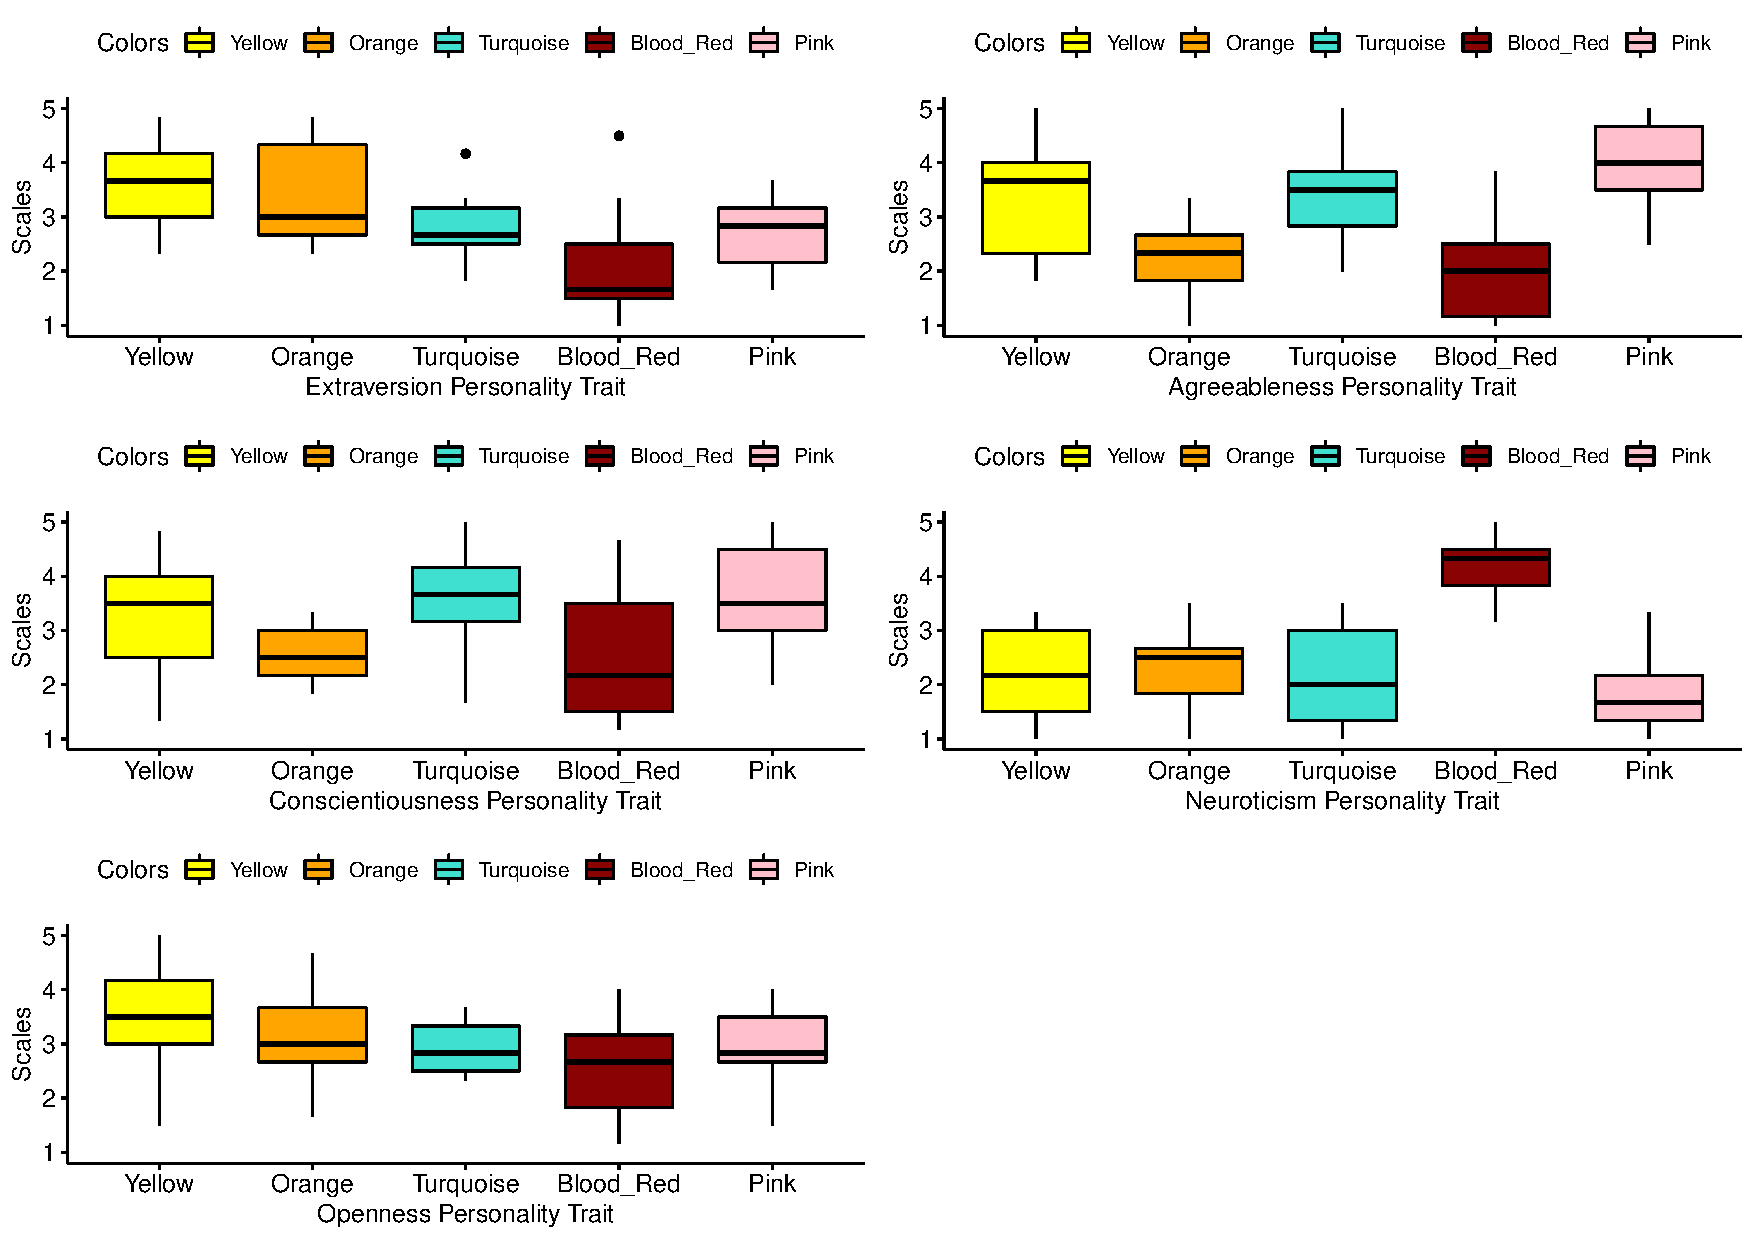
\includegraphics[scale=0.45]{Study1(M-L).pdf}
    \caption{A boxplot for Mascot-Lamp interaction in Study-1}
    \label{fig:ML1}
\end{figure}

%%%%%%%%%%%%%%%%%%%%%%%%%%%%%%%%%%%%%%%%%%%%%%%%%%%%%%%%%%%%%%%%%%%
\subsection{Analysis of within lighting color study}
\label{subsec:MLstudy2}
The second study considers effect of lighting color on how each
personality trait is assessed within one color condition.

\par\textbf{Yellow.}
Friedman test showed a significant difference of the ratings each personality trait
within yellow lighting color with p<0.01, df=4 (see Table~\ref{table:friedmanML2}).
The difference is concentrated on Neuroticism personality which is rated very low when mascot triggers yellow light.
According to Figure~\ref{fig:ML2}, 80\% of scores given for extraversion, agreeableness,
conscientiousness, and openness were higher than all scores given for neurotic personality.
In addition, the similarity of the median values for all personality traits except
neuroticism (Med = 3.7, Med = 3.7, Med = 3.5, Med = 3.5) reveals a small effect of yellow
color on these four personality traits (see Table~\ref{table:medianML2}).

\par\textbf{Orange.}
There is a statistically substantial difference between personality trait measurements within
orange color with p<0.01, df=4 (see Table~\ref{table:friedmanML2}).
When orange color is triggered, the mascot with Extraversion and Openness traits
show distinguishable ratings in comparison to all other personalities with p<0.05 (see Figure~\ref{fig:ML2}).
Moreover, tests did not show any significant differences between extraversion (Med = 3.0, Max = , Min = )
and openness (Med = 3.0, Max = , Min = ) within orange color (see Figure~\ref{fig:ML2} and Table~\ref{table:medianML2}).
However, the median values of extraversion and openness are higher compared to values of all other personality traits.

\par\textbf{Turquoise.}
Overall all personality traits shows different results when light was transformed to turquoise color
with p<0.01, df=4 (see Table~\ref{table:friedmanML2}).
Wilcoxon test reveals that when the turquoise is displayed, the agreeableness and conscientiousness
personality traits are substantially distinguishable from other personality traits with p<0.05 (see Figure~\ref{fig:ML2}).
Both, conscientiousness and agreeableness personalities measured high when Mascot triggers  turquoise color.
However, these two personalities are not distinguishable within turquoise color.
In Spite of that fact, the median value of conscientiousness (Med = 3.7)is slightly higher than
agreeableness (Med = 3.5) (see Table~\ref{table:medianML2}), high p-values indicate that the measurements of
these two personality traits are not differ when turquoise color is triggered.

\par\textbf{Blood-red.}
lighting color reveals significant difference in measurements of all personality traits
with p<0.01, df=4 (see Table~\ref{table:friedmanML2}).
Moreover, according to Figure~\ref{fig:ML2}, there is an excellent separation of neuroticism boxplot from all other personality traits.
Table~\ref{table:medianML2} shows very high median value for Neuroticism compared to other
personality traits with Med = , Min =  and Max = .

\par\textbf{Pink.}
There is a significant difference in rating Mascots' personality when the pink light is
triggered with p<0.01, df=4 (see Table~\ref{table:friedmanML2}).
According to the Figure~\ref{fig:ML2}, pink lighting color shows a significant effect on agreeableness
and conscientiousness with p<0.01 comparing to extraversion, neuroticism and openness personality traits.
Based on the medians reported in Table~\ref{table:medianML2}, agreeableness has the
highest (Med = 4.0) in contrast to the neuroticism which has a lowest value (Med = 1.7).

\begin{longtable}{ |p{1.7cm}| p{1cm}|p{0.5cm}|p{1.7cm}| }
    \captionsetup{width=13.5cm}
    \caption{The results from Friedman test for all Five Personality traits in case of Mascot-Lamp interaction}
    \label{table:friedmanML2} \\
    \hline
    \multicolumn{1}{| c}{\textbf{Personality trait }}
    & \multicolumn{1}{| c}{\textbf{$\chi^2$}}
    & \multicolumn{1}{| c}{\textbf{df}}
    & \multicolumn{1}{| c |}{\textbf{p}}  \\
    \hline
    \endfirsthead
    \multicolumn{4}{c}%
    {\tablename\ \thetable\ -- \textit{Continued from previous page}} \\
    \hline
    \multicolumn{1}{| c}{\textbf{Personality trait }}
    & \multicolumn{1}{| c}{\textbf{$\chi^2$}}
    & \multicolumn{1}{| c}{\textbf{df}}
    & \multicolumn{1}{| c |}{\textbf{p}}  \\
    \hline
    \endhead
    \hline \multicolumn{4}{r}{\textit{Continued on next page}} \\
    \endfoot
    \hline
    \endlastfoot
    Yellow		&23.566	&4	&p<0.01 \\
    Orange		&38.178	&4	&p<0.01\\
    Turquoise		&37.123	&4	&p<0.01 \\
    Blood-red		&45.475	&4	&p<0.01 \\
    Pink			&60.082	&4	&p<0.01 \\
    \hline
\end{longtable}

\begin{table}[H]
    \renewcommand{\arraystretch}{1.2}
    \caption{Some Caption Y is yellow, O is orange \ldots}
    \label{table:medianML2}
    \begin{center}
        \begin{tabular}{p{0.05\textwidth}|
        p{0.025\textwidth}|p{0.025\textwidth}|p{0.025\textwidth}|p{0.025\textwidth}|p{0.025\textwidth}||
        p{0.025\textwidth}|p{0.025\textwidth}|p{0.025\textwidth}|p{0.025\textwidth}|p{0.025\textwidth}||
        p{0.025\textwidth}|p{0.025\textwidth}|p{0.025\textwidth}|p{0.025\textwidth}|p{0.025\textwidth}|}
            \cline{2-16}
            & \multicolumn{5}{c||}{\textbf{Yellow}} & \multicolumn{5}{c||}{\textbf{Orange}}
            & \multicolumn{5}{c|}{\textbf{Turquoise}} \\
            \cline{2-16}
                            & E & A & C & N & O 			    & E & A & C & N & O   	 	& E & A & C & N & O      \\
            \cline{2-16}
            \textbf{Min}  	& 2.3 & 1.8 & 1.3 & 1.0 & 1.5 		& 2.3 & 1.0 & 1.8 & 1.0 & 1.7  	& 1.8 & 2.0 & 1.7 & 1.0 & 2.3  \\
            \textbf{Med} 	& 3.7 & 3.7 & 3.5 & 2.2 & 3.5 		& 3.0 & 2.3 & 2.5 & 2.5 & 3.0  	& 2.7 & 3.5 & 3.7 & 2.0 & 2.8  \\
            \textbf{Max}	& 4.8 & 5.0 & 4.8 & 3.3 & 5.0 		& 4.8 & 3.3 & 3.3 & 3.5 & 4.7  	& 4.2 & 5.0 & 5.0 & 3.5 & 3.7 \\
            \cline{2-16}
            \cline{2-11}
            &  \multicolumn{5}{|c||}{\textbf{Blood-red}} & \multicolumn{5}{|c||}{\textbf{Pink}} \\
            \cline{2-11}
            & E & A & C & N & O 			& E & A & C & N & O     		\\
            \cline{2-11}
            \textbf{Min} 	& 1.0 & 1.0 & 1.2 & 3.2 & 1.2 		& 1.7 & 2.5 & 2.0 & 1.0 & 1.5 	\\
            \textbf{Med}    & 1.7 & 2.0 & 2.2 & 4.3 & 2.7 	    & 2.8 & 4.0 & 3.5 & 1.7 & 2.8 	\\
            \textbf{Max}  	& 4.5 & 3.8 & 4.7 & 5.0 & 4.0 		& 3.7 & 5.0 & 5.0 & 3.3 & 4.0  	\\
            \cline{2-11}
        \end{tabular}
    \end{center}
\end{table}

\begin{figure}[H]
    \centering
    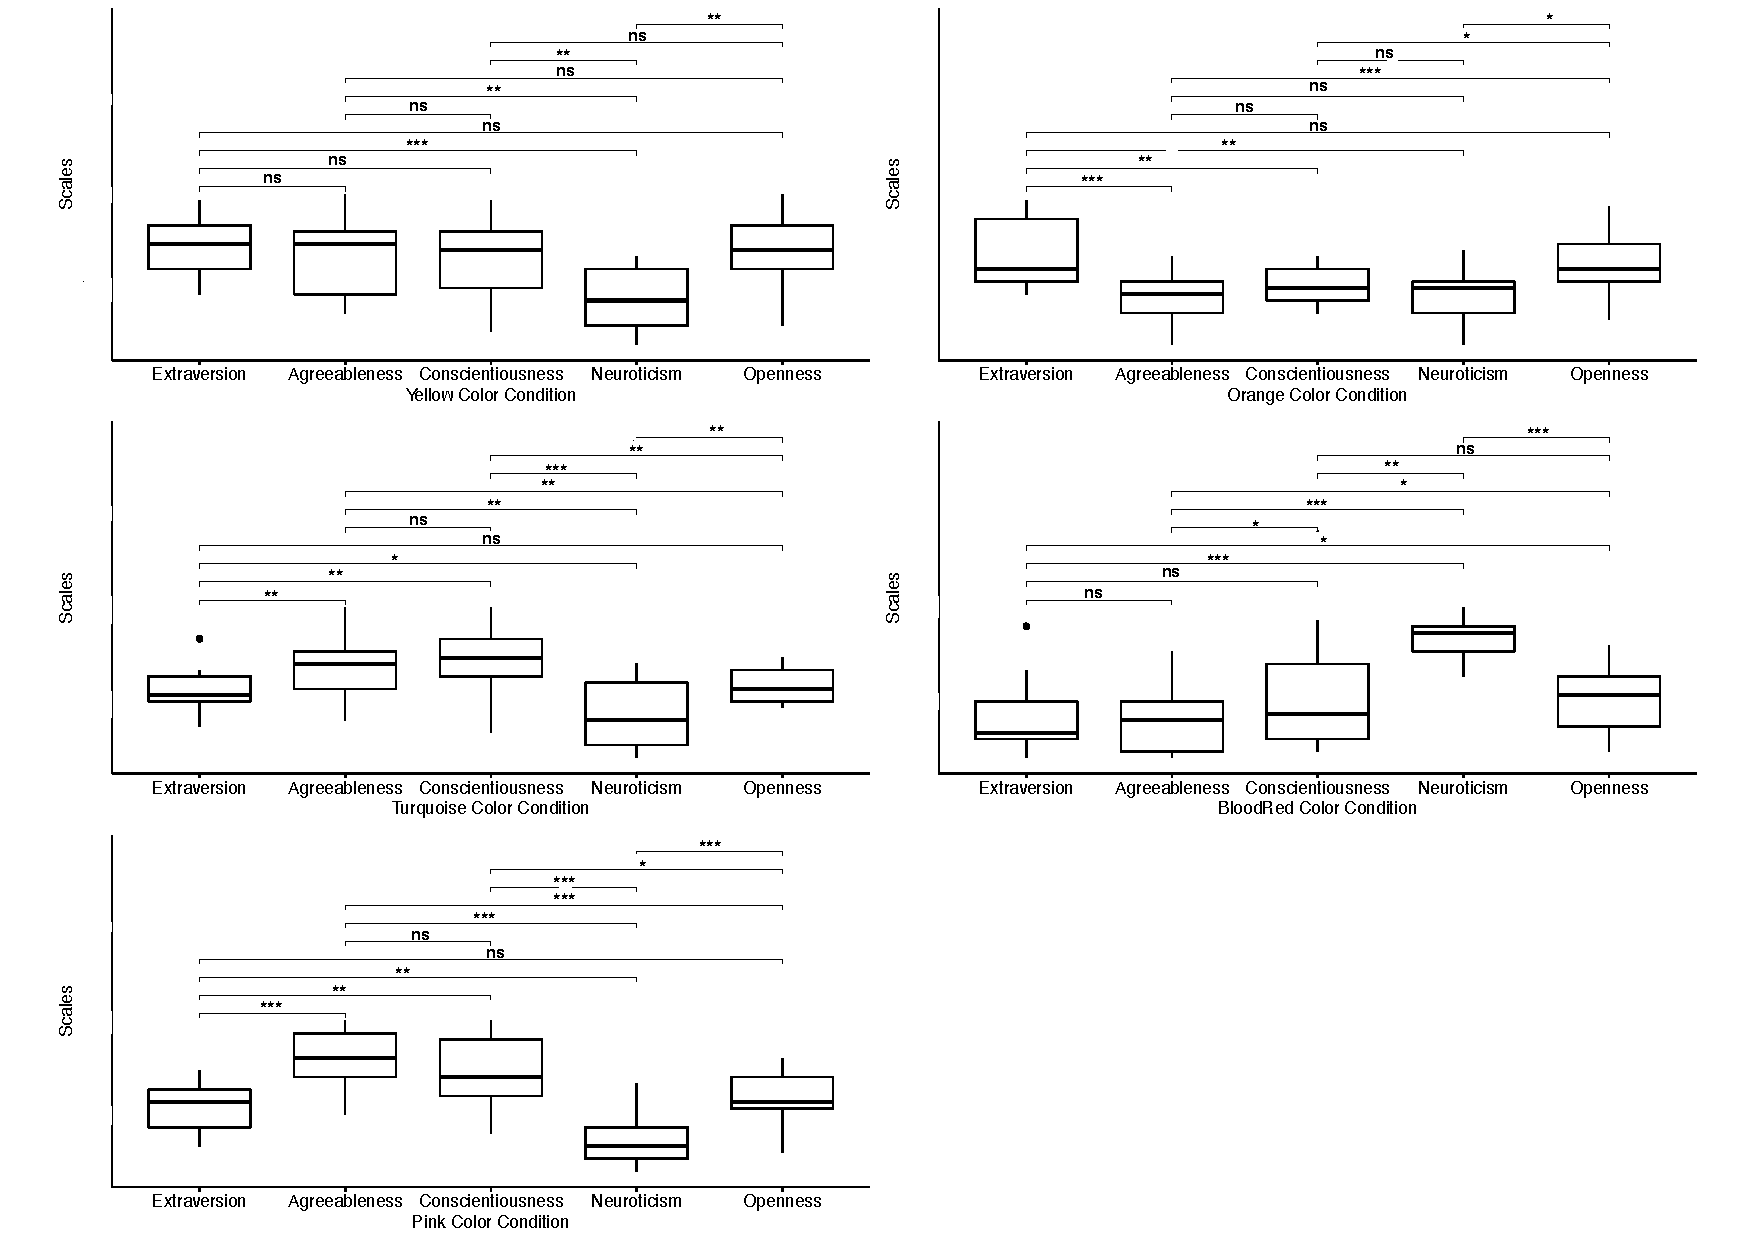
\includegraphics[scale=0.45]{Study2(M-L).pdf}
    \caption{A boxplot for Mascot-Lamp interaction in Study-1}
    \label{fig:ML2}
\end{figure}

%%%%%%%%%%%%%%%%%%%%%%%%%%%%%%%%%%%%%%%%%%%%%%%%%%%%%%%%%%%%%%%%%%%%%%%%%%%%%%%%%%%%%%%%%%%%%%%%%%%%%%%%%%%%%%%%%%%%%%%%
\section{Analysis of Mascot-Speakers interaction}
\label{sec:m-s}
This section includes the Mascot-Speakers case-study, where we analyze the effect music genre
has on the assessment of the Mascots' personality traits.
As we discussed in Chapter~\ref{ch:concept}, our choice of the music genre is based on the MUSIC pattern.
For statistical analysis, we examine the effect of
each category by distributing genres into three categories as the following:
\begin{itemize}
  \item Sophisticated:  jazz, classical and contemporary adult
  \item Contemporary: rap, soul, and rap
  \item Unpretentious: pop, rock\&roll / country and bluegrass
\end{itemize}

The factor that we compare  fo Mascot-Speakers interaction are sophisticated, contemporary and unpretentious music.
In subsection~\ref{subsec:MSstudy1} we analyse within personality trait study,
where we compare the effect of all three music categories on each personality trait.
In subsection~\ref{subsec:MSstudy2}, we compare the same effect within music category.
In case if one music category conveys multiple personality traits, the second study will compare
these traits within that music category and will result in personality with the highest rate.

%%%%%%%%%%%%%%%%%%%%%%%%%%%%%%%%%%%%%%%%%%%%%%%%%%%%%%%%%%%%%%%%%%%
\subsection{Analysis of within personality trait study}
\label{subsec:MSstudy1}
In this subsection, we report a statistical analysis of how the impact of the music category varies within each
personality trait.

\par\textbf{Extraversion.} Table~\ref{table:friedmanMS1}
Friedman tests shows significant effect of all predefined music categories on the
ratings of Extraversion personality with p<0.01, df=2 (see Table~\ref{table:medianMS1}).
Wilcoxon tests revealed that significant difference is concentrated on Contemporary music
with all other categories with padj<0.01 (see Figure~\ref{fig:MS1}).
According to Table~\ref{table:medianMS1}, Contemporary category has the highest median with Med = .

\par\textbf{Agreeableness.}
All these categories significantly influenced participants' measurements of Mascot's
agreeableness personality trait with p<0.01, df=2 (see Table~\ref{table:medianMS1}).
The main difference fault in Sophisticated and Contemporary, and Contemporary
and Unpretentious groups with p<0.01.
According to Figure~\ref{fig:MS1}, it discriminates most of the Contemporary samples from
samples of the other two categories having very low ratings on conveying Agreeableness personality trait.

\par\textbf{Conscientiousness.}
There is a significantly difference of all music categories within conscientiousness
personality trait with p<0.05, df=2 (see Table~\ref{table:medianMS1}.
Similar to Agreeableness personality, when Contemporary music was played, ratings
for Mascot attributing Conscientiousness personality traits were significantly low
in comparison to all other music types with p<0.05, df=2 (see Figure~\ref{fig:MS1}).
Scores for Mascot having Conscientiousness personality traits increased sharply during listening Sophisticated
(median = 3.2) and Unpretentious (median = 3.2) music in comparison to scores for Contemporary music (median = 2.8)
The Wilcoxon test confirms the statistically significant difference between Sophisticated and Contemporary
(padj<0.01), and Unpretentious and Contemporary (padj<0.05) categories.

\par\textbf{Neuroticism.}
Overall all three categories has an effect on the measurement of Mascot's neuroticism
personality with p<0.01, df=2 (see Table~\ref{table:medianMS1}).
Table~\ref{table:medianMS1} shows that the scores given for Contemporary music while assessing
Neuroticism personality traits are highest with Med = 3.1 compared to other two categories.
Moreover, there are two significant differences between Sophisticated and Contemporary,
and Contemporary and Unpretentious music with padj<0.01 (see Figure~\ref{fig:MS1}).

\par\textbf{Openness.}
Table~\ref{table:medianMS1} reveals a substantial difference between all three music types
within openness personality trait.
Particularly, there is a good separation of Sophisticated with median = 3.8 and max = 4.9
from other music categories (see Table~\ref{table:medianMS1}).
The samples for the mascot with a current personality trait are well behaved.
There is a large difference between Sophisticated and Contemporary, and Sophisticated
and Unpretentious which is also confirmed with the Bonferroni correction with p<0.01 (see Figure~\ref{fig:MS1}).

\begin{longtable}{ |p{3cm}| p{1cm}|p{0.5cm}|p{1.7cm}| }
    \captionsetup{width=13.5cm}
    \caption{The results from Friedman test for all Five Personality traits in case of Mascot-Speakers interaction}
    \label{table:friedmanMS1} \\
    \hline
    \multicolumn{1}{| c}{\textbf{Personality trait }}
    & \multicolumn{1}{| c}{\textbf{$\chi^2$}}
    & \multicolumn{1}{| c}{\textbf{df}}
    & \multicolumn{1}{| c |}{\textbf{p}}  \\
    \hline
    \endfirsthead
    \multicolumn{4}{c}%
    {\tablename\ \thetable\ -- \textit{Continued from previous page}} \\
    \hline
    \multicolumn{1}{| c}{\textbf{Personality trait }}
    & \multicolumn{1}{| c}{\textbf{$\chi^2$}}
    & \multicolumn{1}{| c}{\textbf{df}}
    & \multicolumn{1}{| c |}{\textbf{p}}  \\
    \hline
    \endhead
    \hline \multicolumn{4}{r}{\textit{Continued on next page}} \\
    \endfoot
    \hline
    \endlastfoot
    Extraversion		&21.44	&2	&p<0.01 \\
    Agreeableness		&29.01	&2	&p<0.01\\
    Conscientiousness	&6.4536	&2	&p<0.05\\
    Neuroticism		&15.122 	&2	&p<0.01 \\
    Openness			&25.838	&2	&p<0.01 \\
    \hline
\end{longtable}

\begin{table}[H]
    \renewcommand{\arraystretch}{1.2}
    \caption{Some Caption Y is yellow, O is orange \ldots}
    \label{table:medianMS1}
    \begin{center}
        \begin{tabular}{p{0.05\textwidth}|
        p{0.025\textwidth}|p{0.025\textwidth}|p{0.025\textwidth}||
        p{0.025\textwidth}|p{0.025\textwidth}|p{0.025\textwidth}||
        p{0.025\textwidth}|p{0.025\textwidth}|p{0.025\textwidth}||
        p{0.025\textwidth}|p{0.025\textwidth}|p{0.025\textwidth}||
        p{0.025\textwidth}|p{0.025\textwidth}|p{0.025\textwidth}|}
            \cline{2-16}
            & \multicolumn{3}{c||}{\textbf{E}} & \multicolumn{3}{c||}{\textbf{A}}
            & \multicolumn{3}{c||}{\textbf{C}} &  \multicolumn{3}{c||}{\textbf{N}} & \multicolumn{3}{c|}{\textbf{O}} \\
            \cline{2-16}
                            & S & C & U  			& S & C & U   	 	& S & C & U      & S & C & U  		& S & C & U     		\\
            \cline{2-16}
            \textbf{Min}  	& 1.4 & 3.2 & 2.2  		& 2.9 & 1.1 & 2.5   	& 2.4 & 1.0 & 1.9   & 1.0 & 2.3 & 1.3 	& 3.1 & 2.0 & 2.5 \\
            \textbf{Med} 	& 3.1 & 3.9 & 3.3  		& 3.3 & 2.9 & 3.7  	    & 3.2 & 2.8 & 3.2   & 2.4 & 3.1 & 2.5 	& 3.8 & 2.9 & 3.4\\
            \textbf{Max}	& 3.8 & 5.0 & 4.0  		& 4.7 & 4.3 & 4.7   	& 4.6 & 4.0 & 4.7   & 3.4 & 4.5 & 3.2 	& 4.9 & 4.0 & 4.7\\
            \cline{2-16}
        \end{tabular}
    \end{center}
\end{table}

\begin{figure}[H]
    \centering
    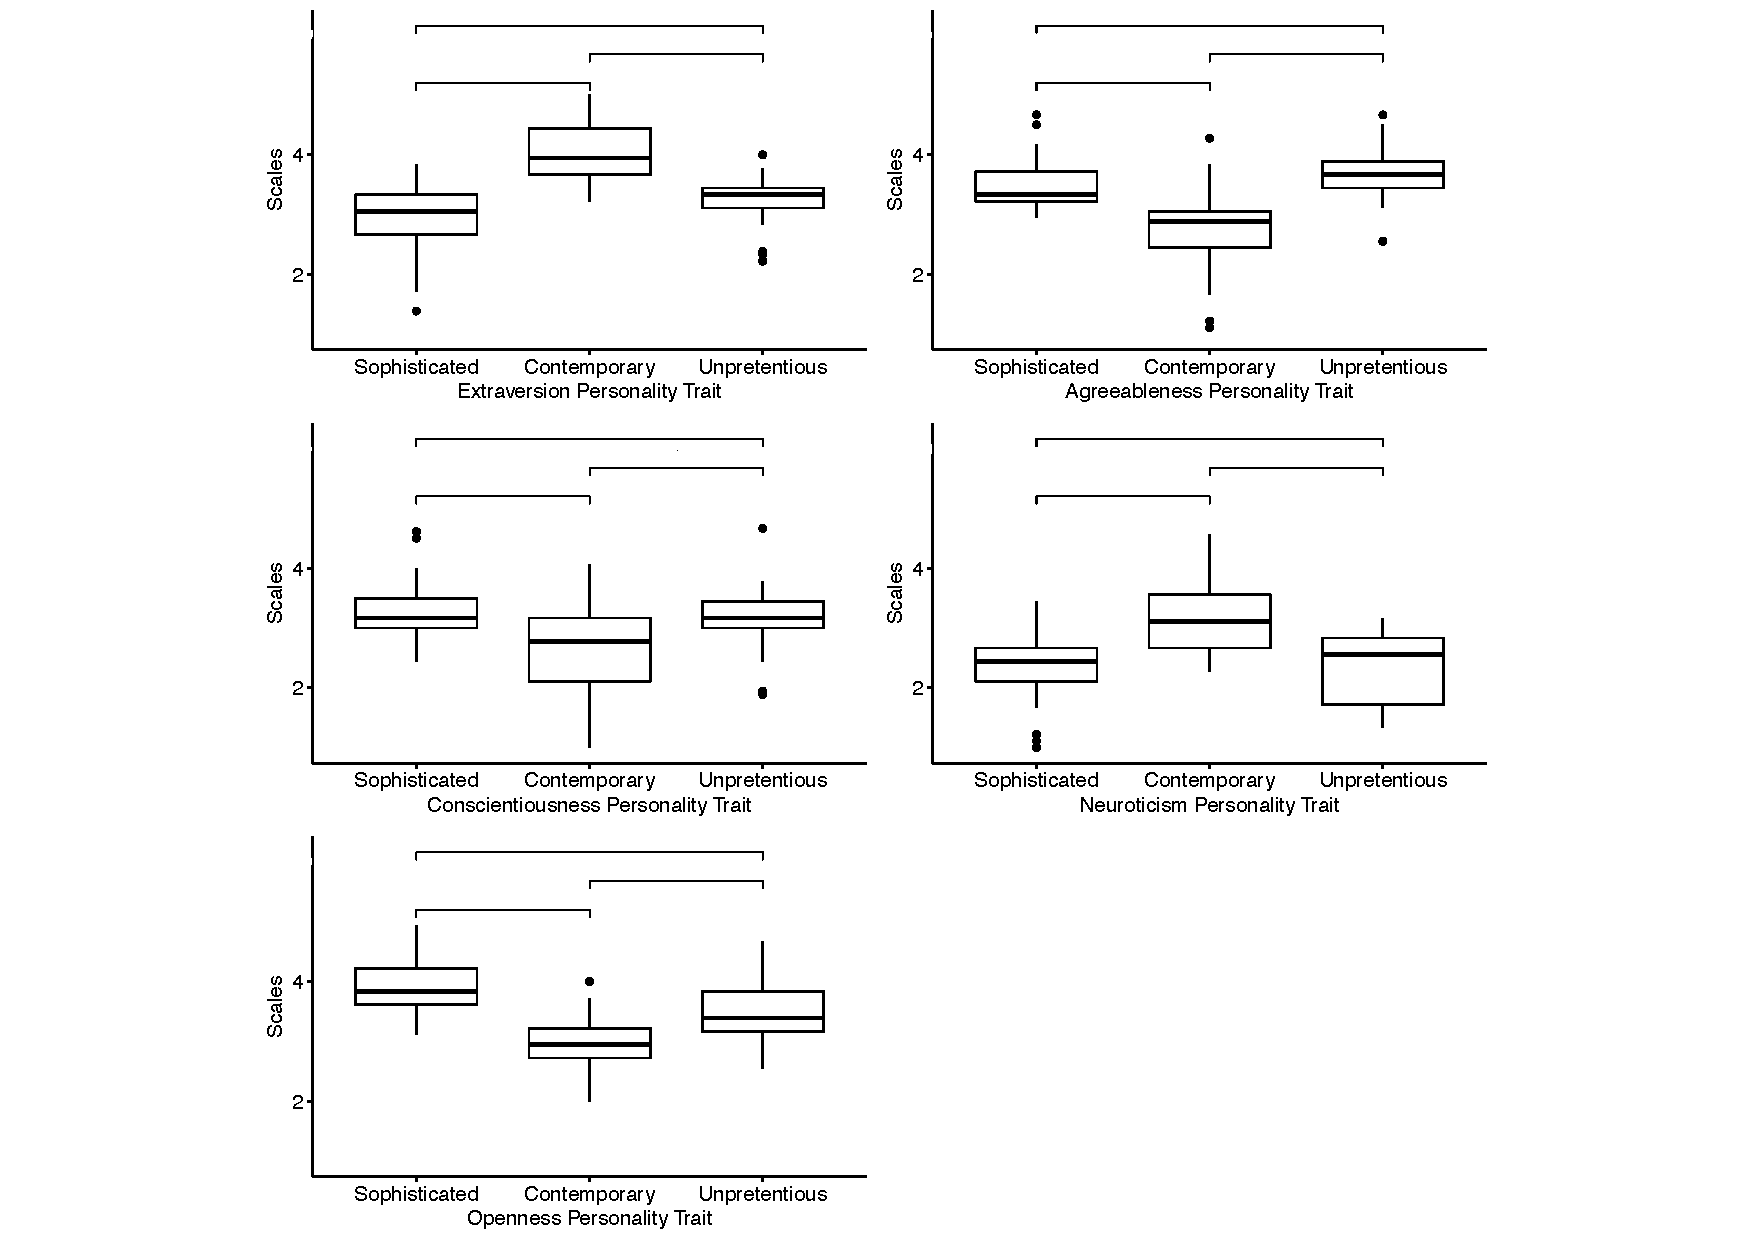
\includegraphics[scale=0.45]{Study1(M-S).pdf}
    \caption{A boxplot for Mascot-Lamp interaction in Study-1}
    \label{fig:MS1}
\end{figure}

%%%%%%%%%%%%%%%%%%%%%%%%%%%%%%%%%%%%%%%%%%%%%%%%%%%%%%%%%%%%%%%%%%%
\subsection{Analysis of within music category study}
\label{subsec:MSstudy2}
In this study, we analyze the effect of each music category, particularly on how each personality
trait is assessed differently within one music condition.

\par\textbf{Sophisticated.}
On average, Sophisticated music has a significant effect on all five personality traits with
p<0.01, df=2 (see Table~\ref{table:friedmanMS2}).
Particularly, this effect is concentrated on Openness personality traits being rated
very high with p<0.01, df=2 (see Table~\ref{table:friedmanMS2}).
When Sophisticated is played, in comparison to all the personality traits, Neuroticism
is rated very low with Med = (see Table~\ref{table:medianMS2}).
Moreover, openness, agreeableness, and neuroticism personality traits shows
significant difference between each other and all other personality traits in the group.

\par\textbf{Contemporary.}
Friedman test shows a significant difference between the ratings of all personality traits and
Contemporary music with p<0.01, df=2 (see Table~\ref{table:friedmanMS2}).
According to the Figure~\ref{fig:MS2}, for Mascot triggering Contemporary music, there is a clear
separation of extraversion samples from all other personality traits with padj<0.01.
The median value for extraversion is very high (Med = 3.9, Max = , Min =) compared to all
other personality traits (Med $\approx$ 3).

\par\textbf{Unpretentious.}
music substantially effected the measurements of all personality traits with
p<0.01, df=4 (see Table~\ref{table:friedmanMS2}).
Based on Wilcoxon tests, neuroticism personality trait is rated very low when Unpretentious music
is played with p < 0.01 (see Figure~\ref{fig:MS2}).
The median values of all other personality traits slightly differ from each other,
condensed around "neutral" rating with Med $\approx$ 3 (see Table~\ref{table:medianMS2})

\begin{longtable}{ |p{2cm}| p{1cm}|p{0.5cm}|p{1.7cm}| }
    \captionsetup{width=13.5cm}
    \caption{The results from Friedman test for all Five Personality traits in case of Mascot-Speakers interaction }
    \label{table:friedmanMS2} \\
    \hline
    \multicolumn{1}{| c}{\textbf{Personality trait }}
    & \multicolumn{1}{| c}{\textbf{$\chi^2$}}
    & \multicolumn{1}{| c}{\textbf{df}}
    & \multicolumn{1}{| c |}{\textbf{p}}  \\
    \hline
    \endfirsthead
    \multicolumn{4}{c}%
    {\tablename\ \thetable\ -- \textit{Continued from previous page}} \\
    \hline
    \multicolumn{1}{| c}{\textbf{Personality trait }}
    & \multicolumn{1}{| c}{\textbf{$\chi^2$}}
    & \multicolumn{1}{| c}{\textbf{df}}
    & \multicolumn{1}{| c |}{\textbf{p}}  \\
    \hline
    \endhead
    \hline \multicolumn{4}{r}{\textit{Continued on next page}} \\
    \endfoot
    \hline
    \endlastfoot
    Sophisticated		&66.573	&4	&p<0.01 \\
    Contemporary		&44.395	&4	&p<0.01\\
    Unpretentious		&57.433	&4	&p<0.01 \\
    \hline
\end{longtable}

\begin{table}[H]
    \renewcommand{\arraystretch}{1.2}
    \caption{Some Caption Y is yellow, O is orange \ldots}
    \label{table:medianMS2}
    \begin{center}
        \begin{tabular}{p{0.05\textwidth}|
        p{0.025\textwidth}|p{0.025\textwidth}|p{0.025\textwidth}|p{0.025\textwidth}|p{0.025\textwidth}||
        p{0.025\textwidth}|p{0.025\textwidth}|p{0.025\textwidth}|p{0.025\textwidth}|p{0.025\textwidth}||
        p{0.025\textwidth}|p{0.025\textwidth}|p{0.025\textwidth}|p{0.025\textwidth}|p{0.025\textwidth}|}
            \cline{2-16}
            & \multicolumn{5}{c||}{\textbf{Sophisticated}} & \multicolumn{5}{c||}{\textbf{Contemporary}}
            & \multicolumn{5}{c|}{\textbf{Unpretentious}} \\
            \cline{2-16}
            & E & A & C & N & O 			    & E & A & C & N & O   	 	& E & A & C & N & O     \\
            \cline{2-16}
            \textbf{Min}  	& 1.4 & 2.9 & 2.4 & 1.0 & 3.1 		& 3.2 & 1.1 & 1.0 & 2.3 & 2.0  	& 2.2 & 2.5 & 1.9 & 1.3 & 2.5  \\
            \textbf{Med} 	& 3.0 & 3.3 & 3.2 & 2.4 & 3.8 		& 3.9 & 2.9 & 2.8 & 3.1 & 2.9  	& 3.3 & 3.7 & 3.2 & 2.5 & 3.4   \\
            \textbf{Max}	& 3.8 & 4.7 & 4.6 & 3.4 & 4.9 		& 5.0 & 4.3 & 4.0 & 4.5 & 4.0  	& 4.0 & 4.7 & 4.7 & 3.2 & 4.7 \\
            \cline{2-16}
        \end{tabular}
    \end{center}
\end{table}

\begin{figure}[H]
    \centering
    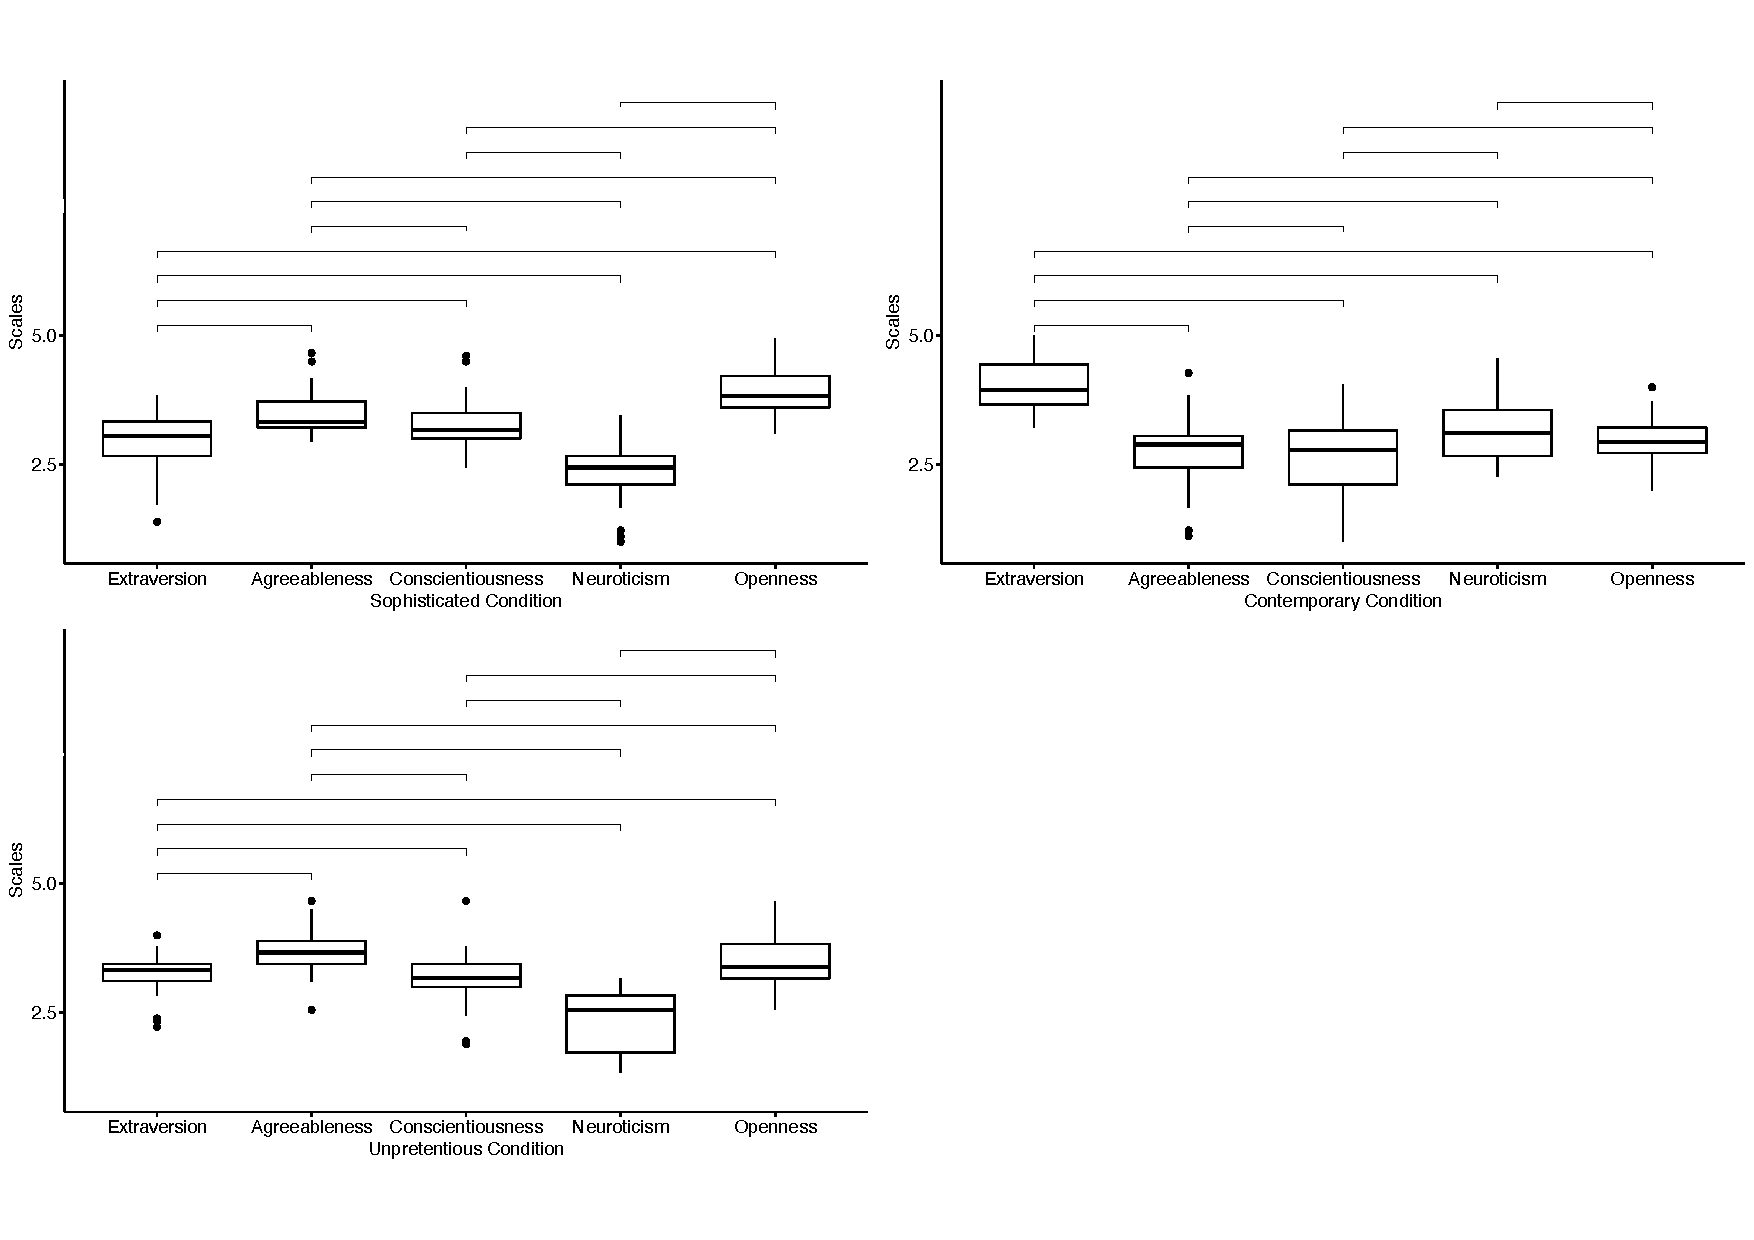
\includegraphics[scale=0.45]{Study2(M-S).pdf}
    \caption{A boxplot for Mascot-Lamp interaction in Study-1}
    \label{fig:MS2}
\end{figure}

%%%%%%%%%%%%%%%%%%%%%%%%%%%%%%%%%%%%%%%%%%%%%%%%%%%%%%%%%%%%%%%%%%%%%%%%%%%%%%%%%%%%%%%%%%%%%%%%%%%%%%%%%%%%%%%%%%%%%%%%
\section{Analysis of Mascot-Mascot interaction}
\label{sec:m-m}
This section covers the analysis of the effect of each level of vibration on the perception
of the personality trait of approaching mascot which triggers this vibration.
The factors that we compare for Mascot-Mascot interaction are five levels of vibration
with a different duration starting from 100 to 500 milliseconds per time.
In Subsection~\ref{subsec:MMstudy1}, we conduct statistical tests for within each
personality trait and in Subsection~\ref{subsec:MMstudy2} for within each vibration level.
In addition, from now on each vibration level is abbreviated accordingly.
For example, the vibration with 500-millisecond duration is abbreviated
as ‘Level-5’, and with 100-millisecond long as ‘Level-1’ and so on.

%%%%%%%%%%%%%%%%%%%%%%%%%%%%%%%%%%%%%%%%%%%%%%%%%%%%%%%%%%%%%%%%%%%
\subsection{Analysis of within personality trait study}
\label{subsec:MMstudy1}
In the first study, we analyse the impact of all vibration levels within each personality trait.
In this study, we analyze each personality trait individually and explore which vibration
level conveys it most.

\par\textbf{Extraversion.}
Friedman test shows significant difference between all levels of vibration in the
ratings of Extraversion personality trait with p<0.01 (see Table~\ref{table:friedmanMM1}).
In comparison to all other levels, Level5 and Level-4 show a significant difference
in the measurements of the extraversion personality with p<0.05 (see Figure~\ref{fig:MM1}).
Both of these levels were highly scored as the behavior of an extravert mascot
with Med = 4.0, for Level-5 and Med = 3.0 for Level-4 (see Table~\ref{table:medianMM1}).

\par\textbf{Agreeableness.}
All vibration levels substantially effected the measurements of Agreeableness personality
trait with p<0.01, df=4 (see Table~\ref{table:friedmanMM1}).

Both Level-2 and Level-3 revealed a significant effect for mascot being
assessed as agreeable with padj < 0.05 (see Figure~\ref{fig:MM1}).
Overall, the majority of votes given for Level-2 (Med = 4.0, Max = , Min = ) and Level-3
(Med = 3.5, Max = , Min = ) attributing agreeableness personality, are higher than most
votes given for other vibration levels (see Table~\ref{table:medianMM1}).

\par\textbf{Conscientiousness.}
There is a significant impact of all vibration levels on the assessment of conscientiousness
personality trait with p<0.01, df=4 (see Table~\ref{table:friedmanMM1}).
The analysis revealed strong impact of levels three abd four on padj < 0.01 (see Figure~\ref{fig:MM1}).
Moreover, the median values for Level-3 (Med = 3.8) and Level-4 (Med = 4.0) are high enough
to show strong impact of these levels to measure mascot as Conscientious (see Table~\ref{table:medianMM1}).

\par\textbf{Neuroticism.}
There is a significant difference of measurements of each level of vibration within Neuroticism
personality trait with p<0.01, df=4 (see Table~\ref{table:friedmanMM1}).
Moreover, especially this difference is concentrated on the ratings for Level-1 with Med = 3.7
in comparison to other levels with Med < 2.5 (see Table~\ref{table:medianMM1}).
For a Neuroticism personality trait, there is a good separation of samples for Level-1
from all other vibration levels with p<0.05 (see Figure~\ref{fig:MM1}).

\par\textbf{Openness.}
Table~\ref{table:friedmanMM1} reveals a difference between all five vibration levels within
openness personality trait with p<0.05, df=4 (see Table~\ref{table:friedmanMM1}).

The Wilcoxon test revealed a significant difference between levels one and two, on
openness personality trait with p < 0.05 (see Figure~\ref{fig:MM1}).
The median values for Level-5, Level4, Level-2, and Level-1 imply the overall
similarity of votes concentrated on the “neutral” scale with Med<2.7 (see Table~\ref{table:medianMM1}).

\begin{longtable}{ |p{3cm}| p{1cm}|p{0.5cm}|p{1.7cm}| }
    \captionsetup{width=13.5cm}
    \caption{The results from Friedman test for all Five Personality traits in case of Mascot-Mascot interaction }
    \label{table:friedmanMM1} \\
    \hline
    \multicolumn{1}{| c}{\textbf{Personality trait }}
    & \multicolumn{1}{| c}{\textbf{$\chi^2$}}
    & \multicolumn{1}{| c}{\textbf{df}}
    & \multicolumn{1}{| c |}{\textbf{p}}  \\
    \hline
    \endfirsthead
    \multicolumn{4}{c}%
    {\tablename\ \thetable\ -- \textit{Continued from previous page}} \\
    \hline
    \multicolumn{1}{| c}{\textbf{Personality trait }}
    & \multicolumn{1}{| c}{\textbf{$\chi^2$}}
    & \multicolumn{1}{| c}{\textbf{df}}
    & \multicolumn{1}{| c |}{\textbf{p}}  \\
    \hline
    \endhead
    \hline \multicolumn{4}{r}{\textit{Continued on next page}} \\
    \endfoot
    \hline
    \endlastfoot
    Extraversion		&30.82	&4	&p<0.01 \\
    Agreeableness		&19.767	&4	&p<0.01 \\
    Conscientiousness	& 43.236	&4	&p<0.01 \\
    Neuroticism		&28.212	&4	&p<0.01\\
    Openness			&11.169	&4	&p<0.05 \\
    \hline
\end{longtable}

\begin{table}[H]
    \renewcommand{\arraystretch}{1.2}
    \caption{Some Caption Y is yellow, O is orange \ldots}
    \label{table:medianMM1}
    \begin{center}
        \begin{tabular}{p{0.05\textwidth}|
        p{0.025\textwidth}|p{0.025\textwidth}|p{0.025\textwidth}|p{0.025\textwidth}|p{0.025\textwidth}||
        p{0.025\textwidth}|p{0.025\textwidth}|p{0.025\textwidth}|p{0.025\textwidth}|p{0.025\textwidth}||
        p{0.025\textwidth}|p{0.025\textwidth}|p{0.025\textwidth}|p{0.025\textwidth}|p{0.025\textwidth}|}
            \cline{2-16}
            & \multicolumn{5}{c||}{\textbf{Extraversion}} & \multicolumn{5}{c||}{\textbf{Agreeableness}}
            & \multicolumn{5}{c|}{\textbf{Conscientiousness}} \\
            \cline{2-16}
            & L-1 & L-2 & L-3 & L-4 & L-5 			    & L-1 & L-2 & L-3 & L-4 & L-5   	 	& L-1 & L-2 & L-3 & L-4 & L-5      \\
            \cline{2-16}
            \textbf{Min}  	& 1.2 & 1.7 & 1.3 & 2.2 & 2.3 		& 1.7 & 2.0 & 2.5 & 1.3 & 1.3  	& 1.7 & 1.5 & 2.8 & 2.2 & 1.7  \\
            \textbf{Med} 	& 2.0 & 2.0 & 2.7 & 3.0 & 4.0 		& 2.5 & 4.0 & 3.5 & 2.8 & 2.7  	& 2.5 & 2.7 & 3.8 & 4.0 & 2.8  \\
            \textbf{Max}	& 3.8 & 4.0 & 4.3 & 4.7 & 4.7 		& 4.0 & 4.7 & 5.0 & 4.0 & 3.8  	& 3.8 & 4.2 & 5.0 & 5.0 & 3.8 \\
            \cline{2-16}
            \cline{2-11}
            &  \multicolumn{5}{|c||}{\textbf{Neuroticism}} & \multicolumn{5}{|c||}{\textbf{Openness}} \\
            \cline{2-11}
            & L-1 & L-2 & L-3 & L-4 & L-5  			& L-1 & L-2 & L-3 & L-4 & L-5     		\\
            \cline{2-11}
            \textbf{Min} 	& 2.0 & 1.3 & 1.3 & 1.0 & 1.0 		& 1.1 & 1.8 & 1.5 & 1.0 & 1.3 	\\
            \textbf{Med}    & 3.7 & 2.1 & 1.8 & 2.2 & 2.3 	    & 2.3 & 2.5 & 3.3 & 2.7 & 2.7 	\\
            \textbf{Max}  	& 4.7 & 3.7 & 4.2 & 3.5 & 3.3 		& 4.2 & 4.5 & 4.3 & 4.5 & 4.0  	\\
            \cline{2-11}
        \end{tabular}
    \end{center}
\end{table}

\begin{figure}[H]
    \centering
    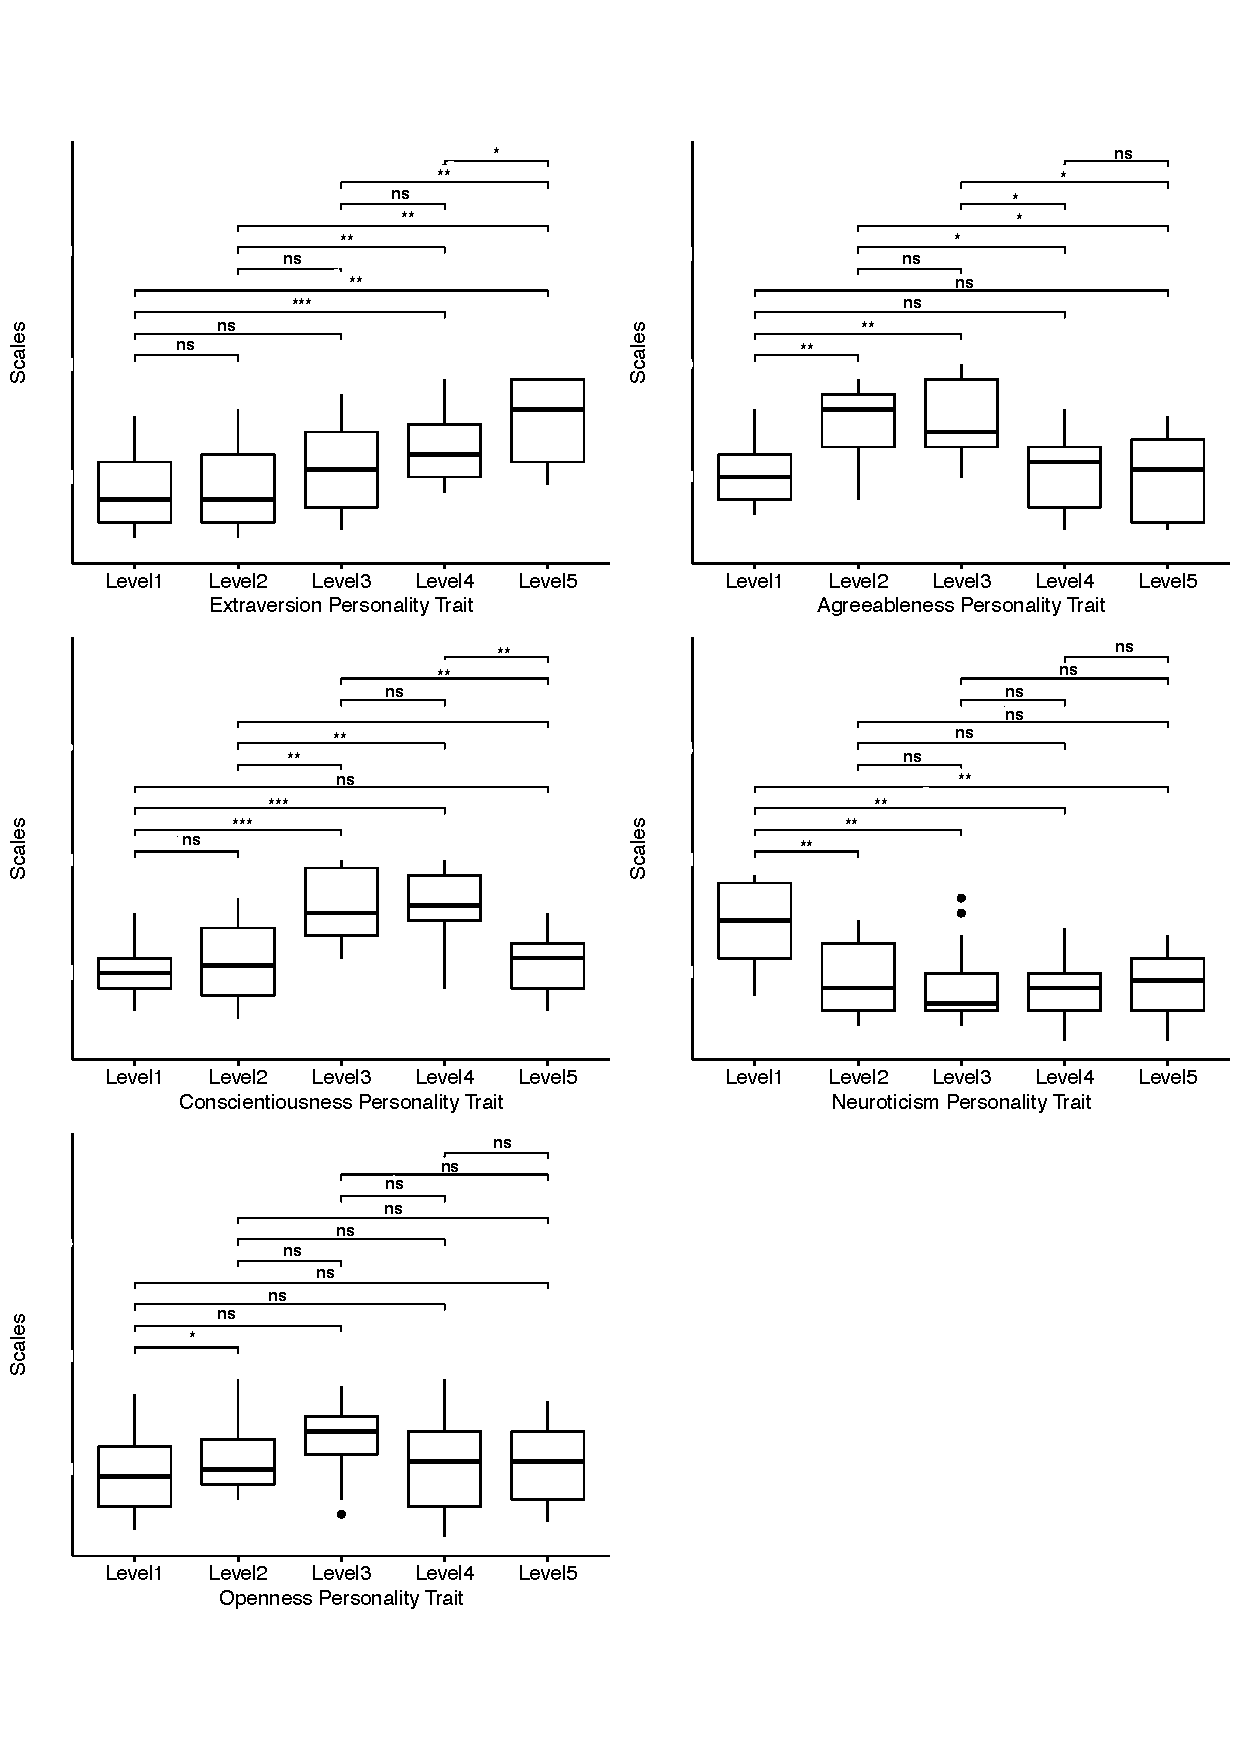
\includegraphics[scale=0.45]{Study1(M-M).pdf}
    \caption{A boxplot for Mascot-Lamp interaction in Study-1}
    \label{fig:MM1}
\end{figure}

%%%%%%%%%%%%%%%%%%%%%%%%%%%%%%%%%%%%%%%%%%%%%%%%%%%%%%%%%%%%%%%%%%%
\subsection{Analysis of within vibration level study}
\label{subsec:MMstudy2}
The second study analyzes each vibration level individually and the difference
of each personality trait within a specific vibration level.

\par\textbf{Level-1.}
Friedman test shows a significant difference between the ratings of all personality traits
and vibration Level-1 with p<0.01, df=4 (see Table~\ref{table:friedmanMM2}).
This difference especially is concentrated on Neuroticism which distinguished it from all
other personality traits with padj<0.05 (see Figure~\ref{fig:}).
In comparison to Neuroticism (Med = 3.7), the median rates given for extraversion,
agreeableness, conscientiousness and openness personality traits are relatively similar,
namely 2.0, 2.5, 2.5, 2.3 respectively (see Table~\ref{table:medianMM2}).

\par\textbf{Level-2.}
On average, Level-2 has a significant effect on the ratings of all five personality
traits with p<0.01, df=4 (see Table~\ref{table:friedmanMM2}).
Based on Wilcoxon tests, there are four groups of personality trait being effected by
vibration Level-2 with padj<0.05 (see Figure~\ref{fig:MM2}).
Moreover, agreeableness is the most distinguishable with being rated higher
than all other personality traits.

\par\textbf{Level-3.}
has a substantial impact on the measurements of personality trait
with p<0.01, df=4 (see Table~\ref{table:friedmanMM2}).
Level-3 effects the ratings of two personality traits: agreeableness and
conscientiousness with padj< 0.05 (see Figure~\ref{fig:MM2}).

\par\textbf{Level-4.}
There is a statistically significant difference between personality trait measurements
with Level-4 with p<0.01, df=4 (see Table~\ref{table:friedmanMM2}).
Level-4 has an impact on the ratings of  two personality traits with the highest scores
such as conscientiousness and extraversion
with a very significant p < 0.01.

\par\textbf{Level-5.}
Overall, all personality traits shows different results when each mascot vibrating 500 milliseconds
per time (i.e Level-5) with p<0.01, df=4 (see Table~\ref{table:friedmanMM2}).
Level-5 distinguishes Exraversion from all other personality traits having the
highest ratings with padj<0.05 (see Figure~\ref{fig:MM2}).
The median values for all other personality traits are lower than neutral scale (Med < 3.0)
in comparison to neuroticism with Med = 4.0 (see Table~\ref{table:medianMM2}).

\begin{longtable}{ |p{2cm}| p{1cm}|p{0.5cm}|p{1.7cm}| }
    \captionsetup{width=13.5cm}
    \caption{The results from Friedman test for all Five Personality traits in case of Mascot-Mascot interaction}
    \label{table:friedmanMM2} \\
    \hline
    \multicolumn{1}{| c}{\textbf{Personality trait }}
    & \multicolumn{1}{| c}{\textbf{$\chi^2$}}
    & \multicolumn{1}{| c}{\textbf{df}}
    & \multicolumn{1}{| c |}{\textbf{p}}  \\
    \hline
    \endfirsthead
    \multicolumn{4}{c}%
    {\tablename\ \thetable\ -- \textit{Continued from previous page}} \\
    \hline
    \multicolumn{1}{| c}{\textbf{Personality trait }}
    & \multicolumn{1}{| c}{\textbf{$\chi^2$}}
    & \multicolumn{1}{| c}{\textbf{df}}
    & \multicolumn{1}{| c |}{\textbf{p}}  \\
    \hline
    \endhead
    \hline \multicolumn{4}{r}{\textit{Continued on next page}} \\
    \endfoot
    \hline
    \endlastfoot
    Level-1		&24.008	&4	&p<0.01 \\
    Level-2		&24.525	&4	&p<0.01 \\
    Level-3		&35.165	&4	&p<0.01 \\
    Level-4		&46.603	&4	&p<0.01 \\
    Level-5		&24.1	&4	&p<0.01 \\
    \hline
\end{longtable}

\begin{table}[H]
    \renewcommand{\arraystretch}{1.2}
    \caption{Some Caption Y is yellow, O is orange \ldots}
    \label{table:medianMM2}
    \begin{center}
        \begin{tabular}{p{0.05\textwidth}|
        p{0.025\textwidth}|p{0.025\textwidth}|p{0.025\textwidth}|p{0.025\textwidth}|p{0.025\textwidth}||
        p{0.025\textwidth}|p{0.025\textwidth}|p{0.025\textwidth}|p{0.025\textwidth}|p{0.025\textwidth}||
        p{0.025\textwidth}|p{0.025\textwidth}|p{0.025\textwidth}|p{0.025\textwidth}|p{0.025\textwidth}|}
            \cline{2-16}
            & \multicolumn{5}{c||}{\textbf{Level-1}} & \multicolumn{5}{c||}{\textbf{Level-2}}
            & \multicolumn{5}{c|}{\textbf{Level-3}} \\
            \cline{2-16}
            & E & A & C & N & O  			    & E & A & C & N & O   	 	& E & A & C & N & O      \\
            \cline{2-16}
            \textbf{Min}  	& 1.2 & 1.7 & 1.7 & 2.0 & 1.2 		& 1.2 & 2.0 & 1.5 & 1.3 & 1.8  	& 1.3 & 2.5 & 2.8 & 1.3 & 1.5  \\
            \textbf{Med} 	& 2.0 & 2.5 & 2.5 & 3.7 & 2.3 		& 2.0 & 4.0 & 2.7 & 2.2 & 2.5  	& 2.7 & 3.5 & 3.8 & 1.8 & 3.3  \\
            \textbf{Max}	& 3.8 & 4.0 & 3.8 & 4.7 & 4.2 		& 4.0 & 4.7 & 4.2 & 3.7 & 4.5  	& 4.3 & 5.0 & 5.0 & 4.2 & 4.3 \\
            \cline{2-16}
            \cline{2-11}
            &  \multicolumn{5}{|c||}{\textbf{Level-4}} & \multicolumn{5}{|c||}{\textbf{Level-5}} \\
            \cline{2-11}
            & E & A & C & N & O  			& E & A & C & N & O     		\\
            \cline{2-11}
            \textbf{Min} 	& 2.2 & 1.3 & 2.2 & 1.0 & 1.0 		& 2.3 & 1.3 & 1.7 & 1.0 & 1.3 	\\
            \textbf{Med}    & 3.0 & 2.8 & 4.0 & 2.2 & 2.7 	    & 4.0 & 2.7 & 2.8 & 2.3 & 2.7 	\\
            \textbf{Max}  	& 4.7 & 4.0 & 5.0 & 3.5 & 4.5 		& 4.7 & 3.8 & 3.8 & 3.3 & 4.0  	\\
            \cline{2-11}
        \end{tabular}
    \end{center}
\end{table}

\begin{figure}[H]
    \centering
    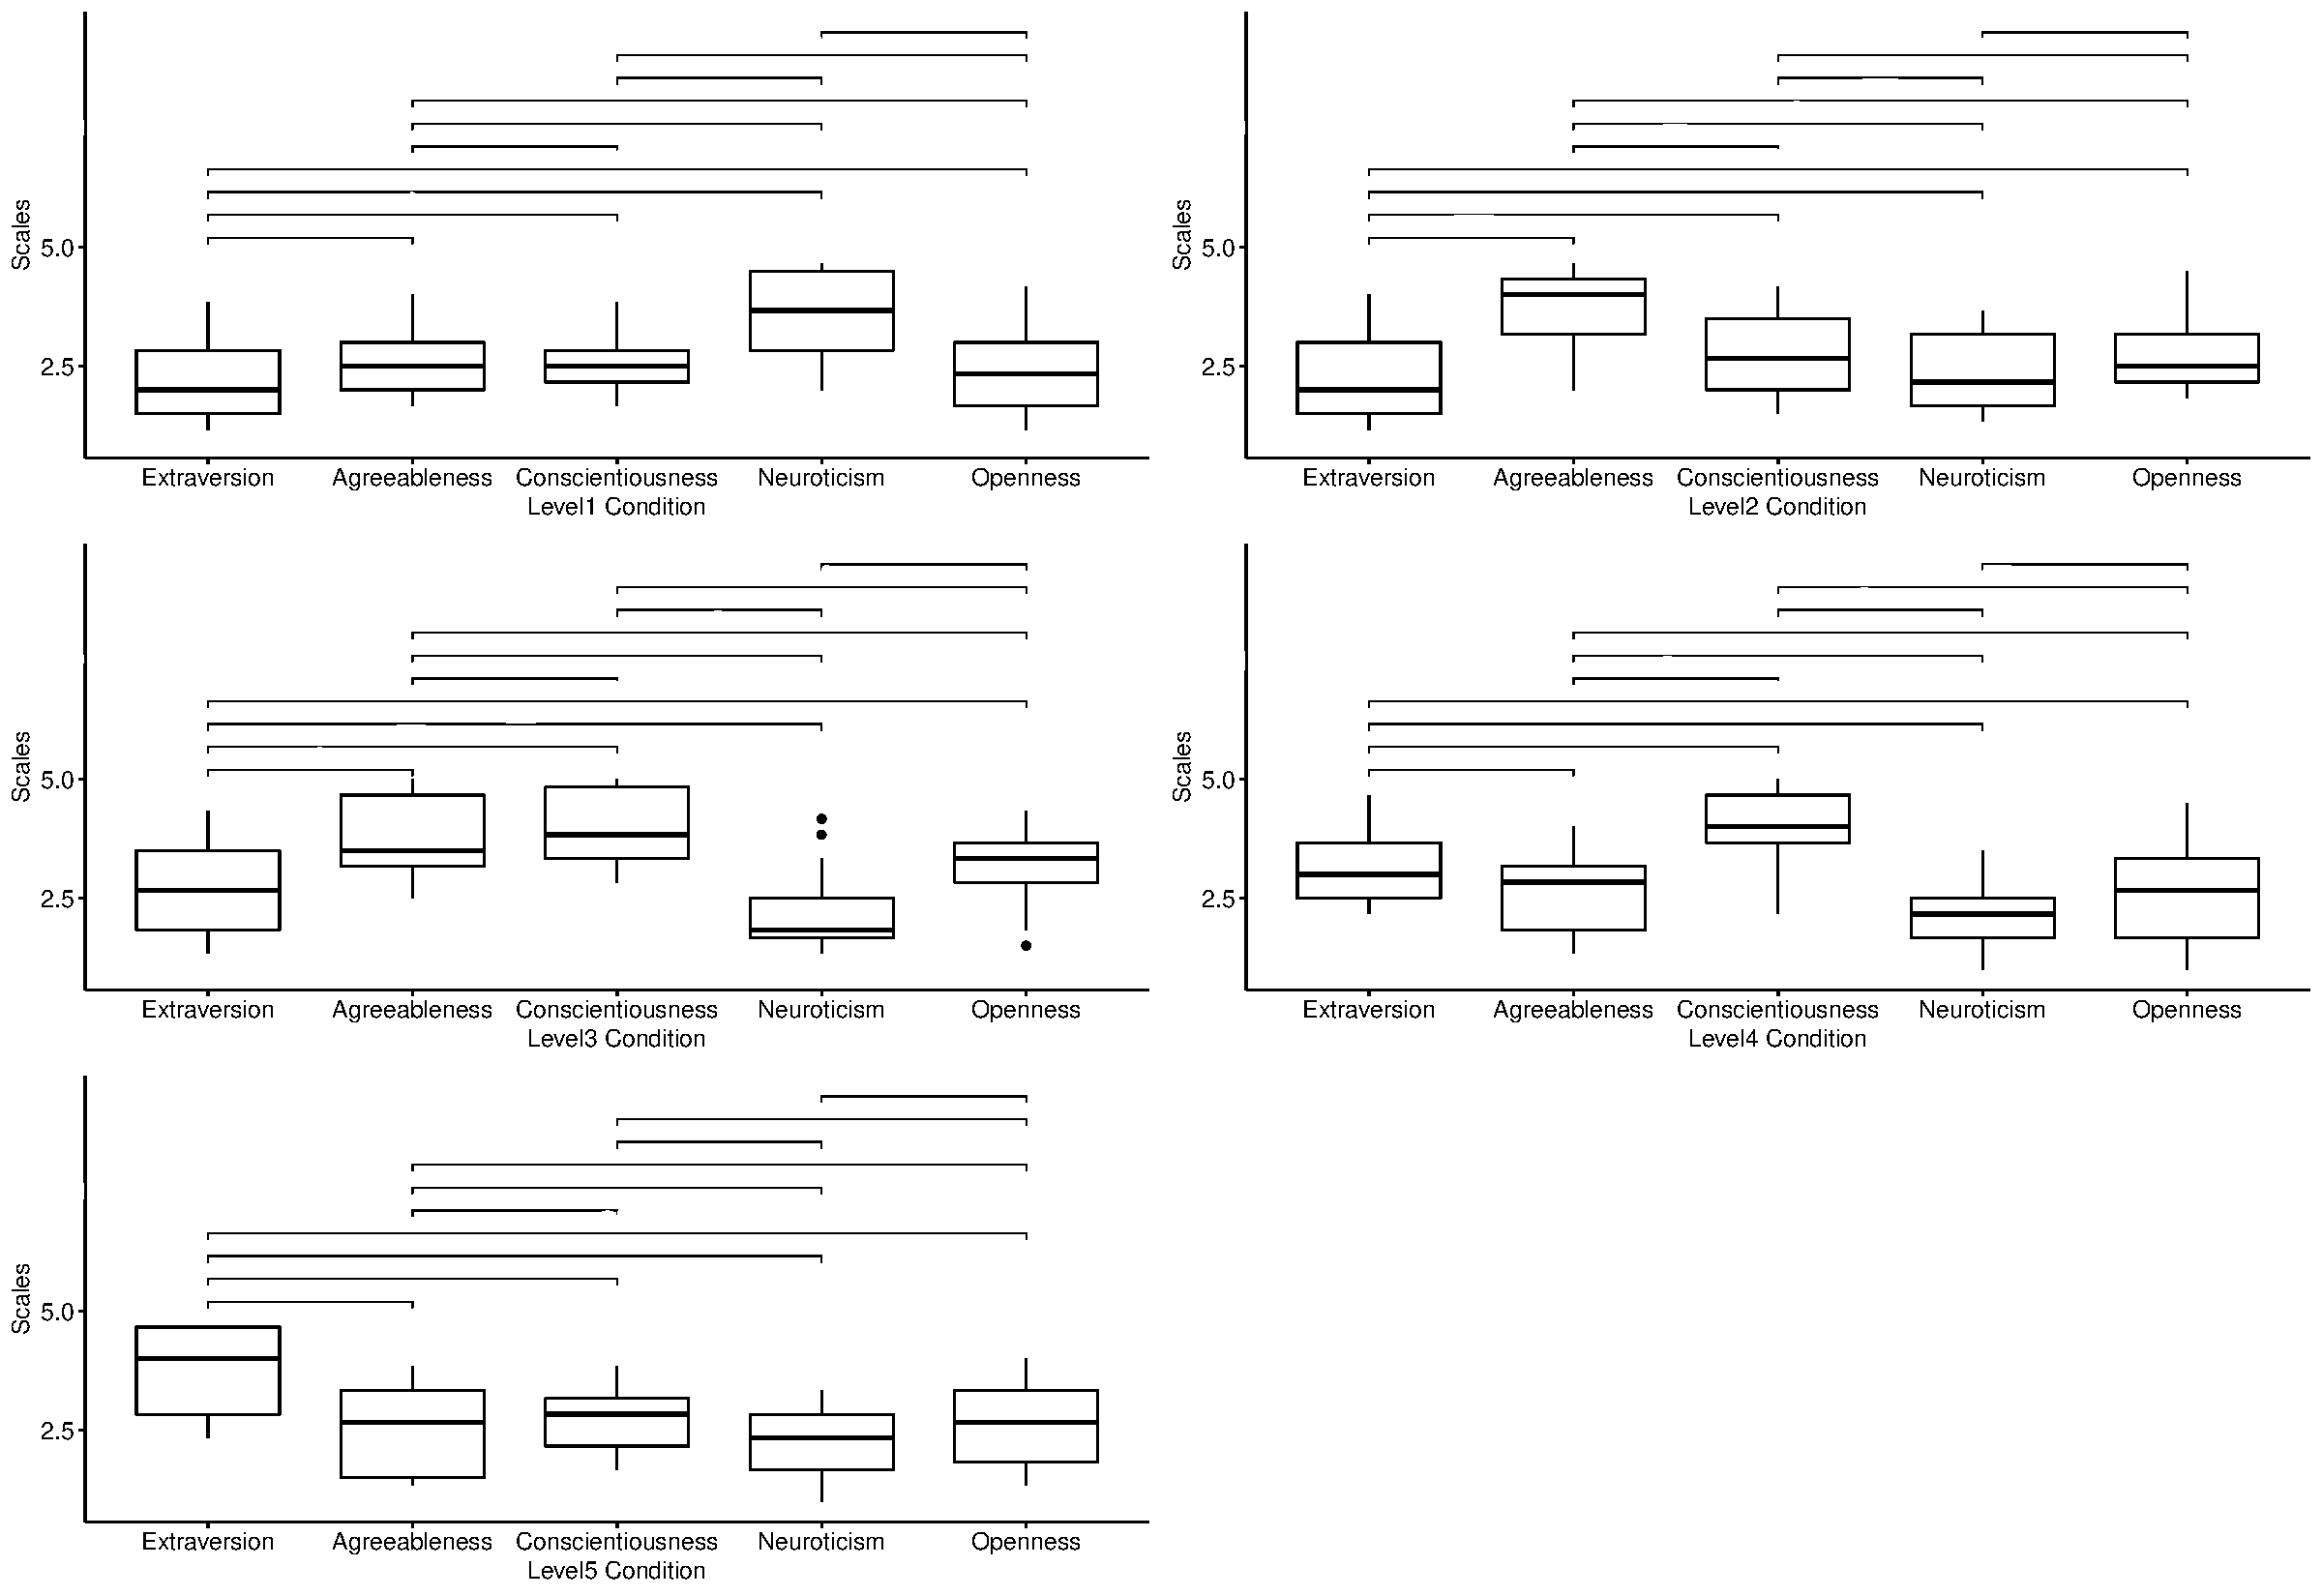
\includegraphics[scale=0.45]{Study2(M-M).pdf}
    \caption{A boxplot for Mascot-Lamp interaction in Study-1}
    \label{fig:MM2}
\end{figure}

%%%%%%%%%%%%%%%%%%%%%%%%%%%%%%%%%%%%%%%%%%%%%%%%%%%%%%%%%%%%%%%%%%%%%%%%%%%%%%%%%%%%%%%%%%%%%%%%%%%%%%%%%%%%%%%%%%%%%%%%
\section{Analysis of Mascot-Tablet interaction}
\label{sec:m-t}
The section describes the impact of the screen color of a tablet on the assessment of the personality trait that
mascot was assigned.
The factors that we compare for Mascot-Tablet interaction are yellow,
orange, turquoise, blood-red and pink screen colors.
Subsection~\ref{subsec:MTstudy1} shows the analysis of within personality study and Subsection~\ref{subsec:MTstudy2} of condition study (i.e color)

%%%%%%%%%%%%%%%%%%%%%%%%%%%%%%%%%%%%%%%%%%%%%%%%%%%%%%%%%%%%%%%%%%%
\subsection{Analysis of within personality trait study}
\label{subsec:MTstudy1}
In our first study, we focus on each personality by comparing the scores given
for each color within that personality trait.

\par\textbf{Extraversion.}
For the measurements of extraversion personality,
the most significant difference was observed when comparing yellow, orange with
blood-red, pink colors with padj<0.05.
Meaning that colors with padj<0.05 shows that samples from yellow and orange colors are separated
from blood-red and pink samples (see Figure~\ref{fig:MT1}).
Moreover, in comparison to other colors most samples for orange are concentrated around
an “accurate” score (Med = 4.2, Max = 5.0) (see Table~\ref{table:medianMT1}).

\par\textbf{Agreeableness.}
Change in tablet's screen color significantly influenced the participants' ratings of
Agreeableness personality trait with p<0.01, df=4 (see Table~\ref{table:friedmanMT1}).
Figure~\ref{fig:MT1}) shows a good separation of turquoise and pink colors
from all others implying that there is a difference in ratings the
agreeableness personality traits having padj < 0.01.
However, there is no strong difference between turquoise and pink colors with
the same value Med = 3.7 (see Table~\ref{table:medianMT1}).

\par\textbf{Conscientiousness.}
There is a significant difference in the rating of Conscientiousness personality trait
when comparing screen colors with p<0.01, df=4 (see Table~\ref{table:friedmanMT1}).
According to Figure~\ref{fig:MT1}, there is a significant difference for
tablet displaying turquoise color in rating mascot as conscientiousness with padj < 0.05.
The median values for yellow (Med = 2.7), pink (Med = 2.8) and orange (Med = 2.7) colors are
concentrated around the “neutral” scale, whereas turquoise (Med = 4.2) (see Table~\ref{table:medianMT1}).

\par\textbf{Neuroticism.}
All predefined screen colors substantially effected the measurements of Neuroticism personality
trait with p<0.01, df=4 (see Table~\ref{table:friedmanMT1}).
According to Figure~\ref{fig:MT1}, there is a great separation of blood-red
samples from all other screen colors.
Moreover, there is a significant difference in the rating of Neuroticism when comparing
Blood-red with other screen colors with padj<0.05.
The rating for blood-red is higher with Med = 3.8 compared to all other colors
being rated low with M $\leq$ 2.5 (see Table~\ref{table:medianMT1}).

\par\textbf{Openness.}
Table~\ref{table:friedmanMT1} shows the different rating based on all colors within openness
personality trait with p<0.01, df=4 (see Table~\ref{table:friedmanMT1}).
According to the Wilcoxon tests, during the measurements of a mascot's 'openness to experience'
personality trait, the yellow is significantly different from all other screen
colors with padj < 0.05 (see Figure~\ref{fig:MT1}).
In comparison to all other colors (M $\leq$ 3.0), most of the samples of yellow color are discriminated
from all others concentrating around an “accurate” scale with a Med = 4.0 (see Table~\ref{table:medianMT1}).

\begin{longtable}{ |p{2.7cm}| p{1cm}|p{0.5cm}|p{1.7cm}| }
    \captionsetup{width=13.5cm}
    \caption{The results from Friedman test for all Five Personality traits in case of Mascot-Tablet interaction}
    \label{table:friedmanMT1} \\
    \hline
    \multicolumn{1}{| c}{\textbf{Personality trait }}
    & \multicolumn{1}{| c}{\textbf{$\chi^2$}}
    & \multicolumn{1}{| c}{\textbf{df}}
    & \multicolumn{1}{| c |}{\textbf{p}}  \\
    \hline
    \endfirsthead
    \multicolumn{4}{c}%
    {\tablename\ \thetable\ -- \textit{Continued from previous page}} \\
    \hline
    \multicolumn{1}{| c}{\textbf{Personality trait }}
    & \multicolumn{1}{| c}{\textbf{$\chi^2$}}
    & \multicolumn{1}{| c}{\textbf{df}}
    & \multicolumn{1}{| c |}{\textbf{p}}  \\
    \hline
    \endhead
    \hline \multicolumn{4}{r}{\textit{Continued on next page}} \\
    \endfoot
    \hline
    \endlastfoot
    Extraversion		&28.841	&4	&p<0.01 \\
    Agreeableness		&52.895	&4	&p<0.01 \\
    Conscientiousness	&32.891	&4	&p<0.01 \\
    Neuroticism		&30.466	&4	&p<0.01 \\
    Openness			&37.725	&4	&p<0.01 \\
    \hline
\end{longtable}

\begin{table}[H]
    \renewcommand{\arraystretch}{1.2}
    \caption{Some Caption Y is yellow, O is orange \ldots}
    \label{table:medianMT1}
    \begin{center}
        \begin{tabular}{p{0.05\textwidth}|
        p{0.025\textwidth}|p{0.025\textwidth}|p{0.025\textwidth}|p{0.025\textwidth}|p{0.025\textwidth}||
        p{0.025\textwidth}|p{0.025\textwidth}|p{0.025\textwidth}|p{0.025\textwidth}|p{0.025\textwidth}||
        p{0.025\textwidth}|p{0.025\textwidth}|p{0.025\textwidth}|p{0.025\textwidth}|p{0.025\textwidth}|}
            \cline{2-16}
            & \multicolumn{5}{c||}{\textbf{Extraversion}} & \multicolumn{5}{c||}{\textbf{Agreeableness}}
            & \multicolumn{5}{c|}{\textbf{Conscientiousness}} \\
            \cline{2-16}
            & Y & O & T & B & P 			    & Y & O & T & B & P  	 	& Y & O & T & B & P     \\
            \cline{2-16}
            \textbf{Min}  	& 2.0 & 1.7 & 2.0 & 1.2 & 1.7 		& 1.5 & 1.2 & 1.8 & 1.0 & 1.7  	& 1.8 & 2.2 & 2.0 & 1.0 & 2.0  \\
            \textbf{Med} 	& 3.3 & 4.2 & 2.8 & 1.7 & 2.5 		& 3.0 & 2.3 & 3.7 & 1.8 & 3.7  	& 2.7 & 2.7 & 4.2 & 2.3 & 2.8  \\
            \textbf{Max}	& 4.0 & 5.0 & 4.3 & 4.7 & 3.8 		& 3.7 & 4.5 & 4.2 & 3.3 & 5.0  	& 3.5 & 4.5 & 5.0 & 4.3 & 4.7 \\
            \cline{2-16}
            \cline{2-11}
            &  \multicolumn{5}{|c||}{\textbf{Neuroticism}} & \multicolumn{5}{|c||}{\textbf{Openness}} \\
            \cline{2-11}
            & Y & O & T & B & P 			& Y & O & T & B & P    		\\
            \cline{2-11}
            \textbf{Min} 	& 1.3 & 1.5 & 1.0 & 1.5 & 1.2 		& 2.5 & 1.3 & 2.0 & 1.0 & 1.5 	\\
            \textbf{Med}    & 2.2 & 2.5 & 2.5 & 3.8 & 2.3 	    & 4.0 & 3.0 & 3.0 & 2.7 & 2.7 	\\
            \textbf{Max}  	& 3.7 & 4.3 & 3.5 & 5.0 & 4.2 		& 5.0 & 5.0 & 4.2 & 3.8 & 3.8  	\\
            \cline{2-11}
        \end{tabular}
    \end{center}
\end{table}

\begin{figure}[H]
    \centering
    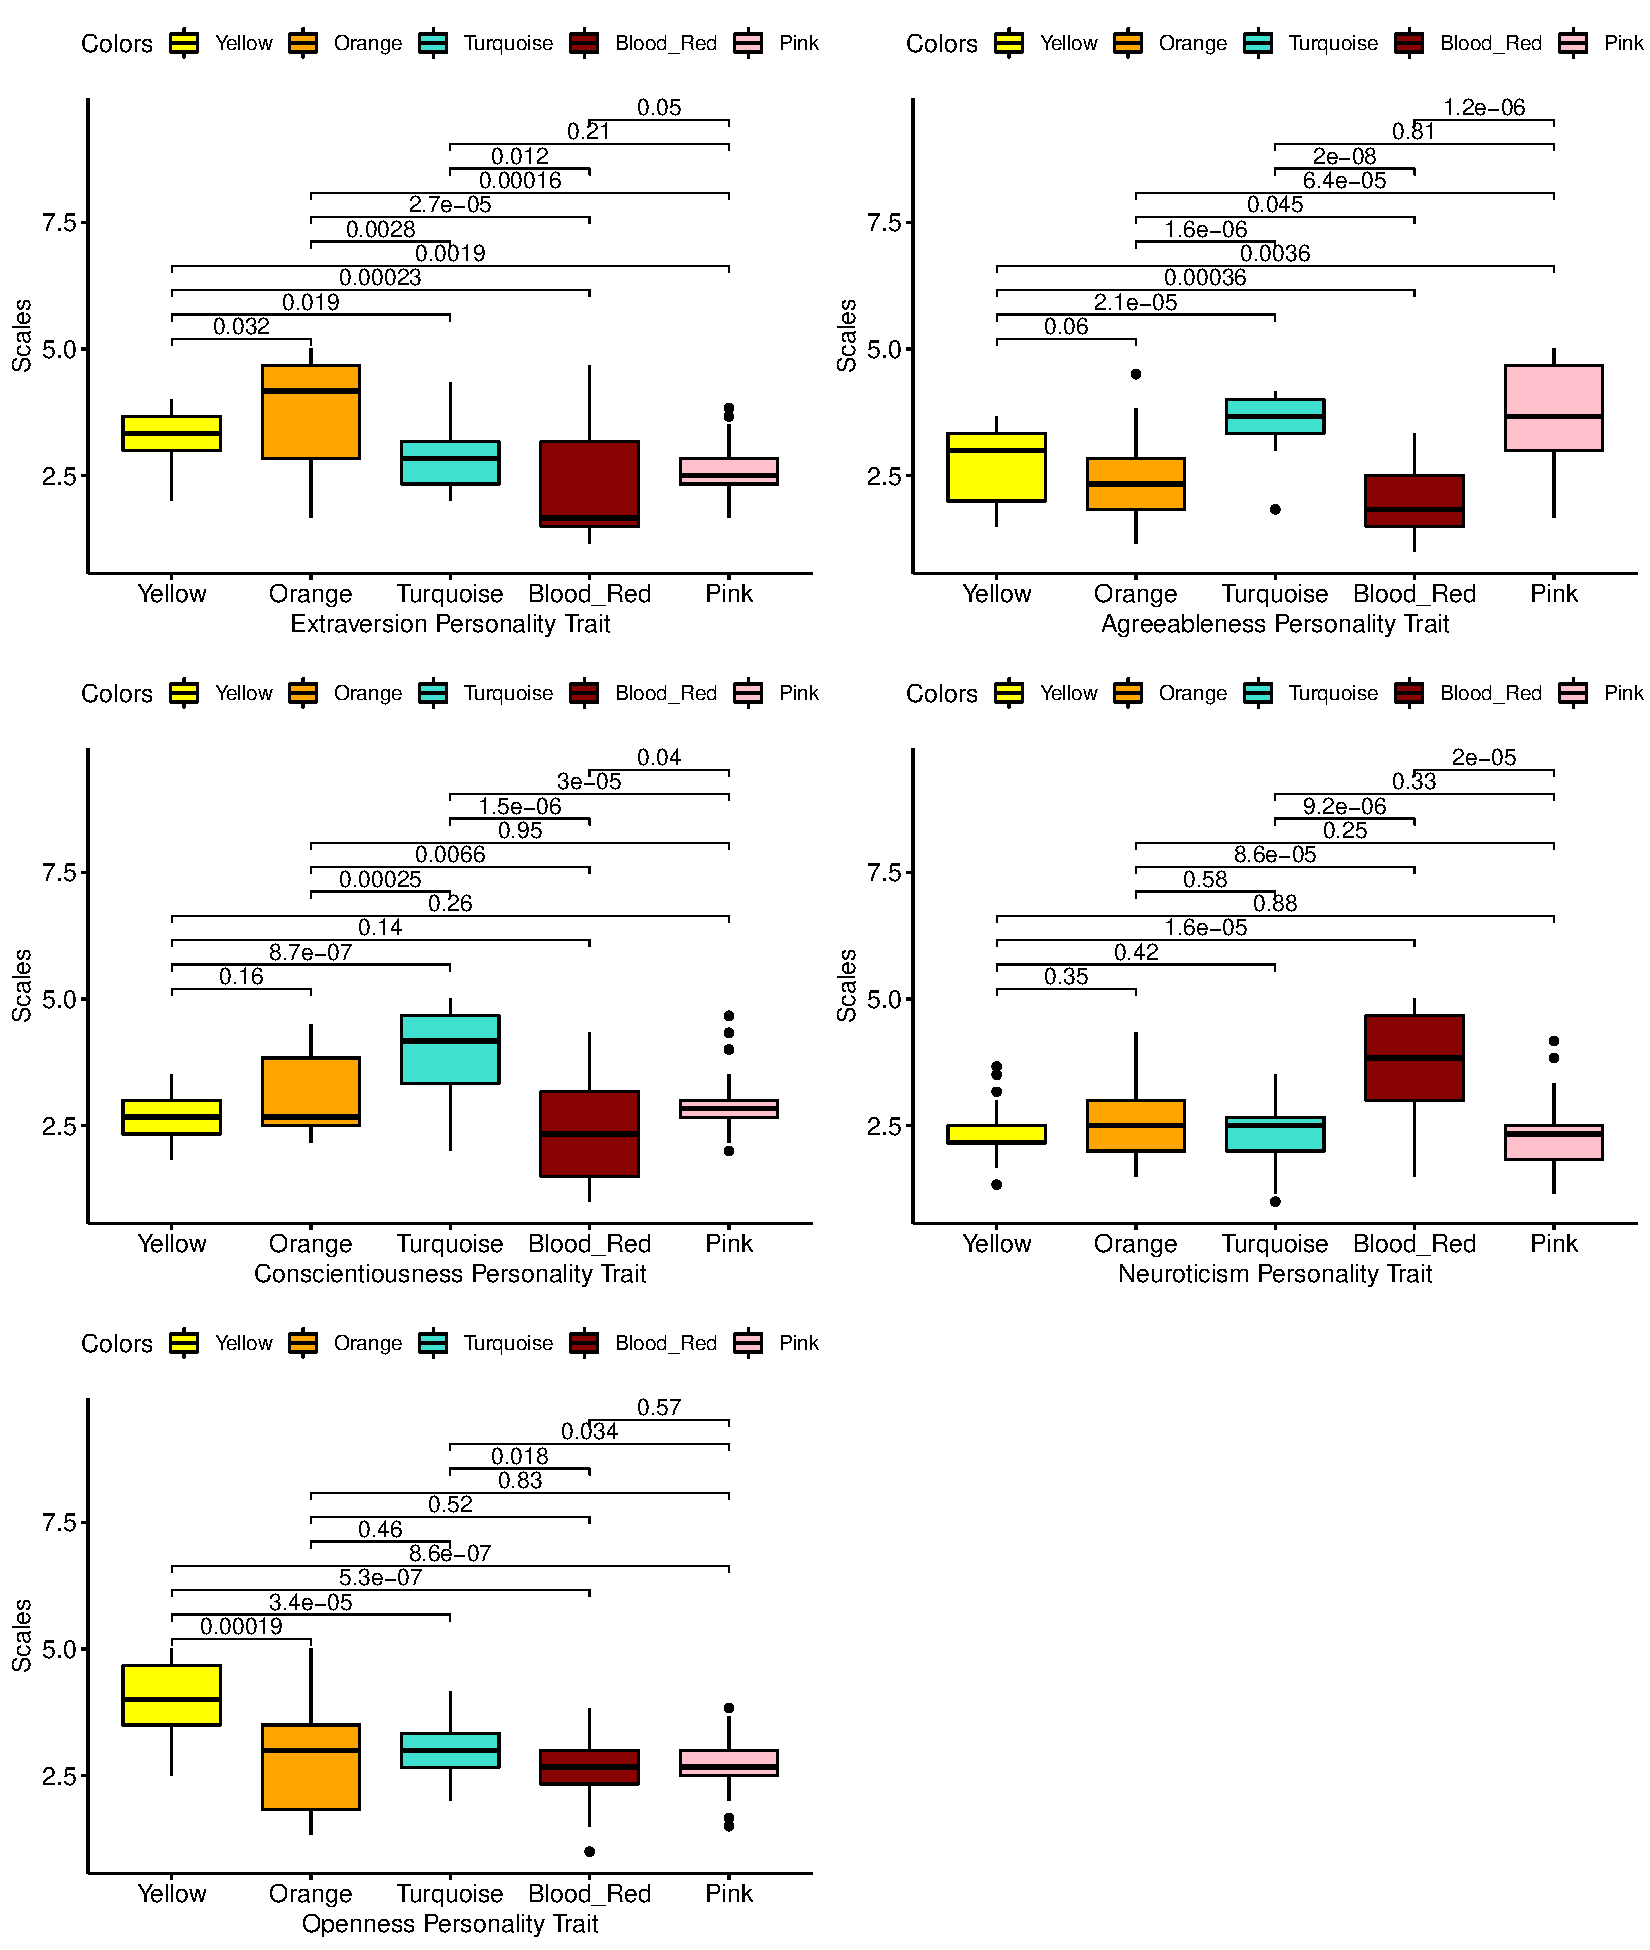
\includegraphics[scale=0.45]{Study1(M-T).pdf}
    \caption{A boxplot for Mascot-Lamp interaction in Study-1}
    \label{fig:MT1}
\end{figure}

\par\textbf{Extraversion.}

%%%%%%%%%%%%%%%%%%%%%%%%%%%%%%%%%%%%%%%%%%%%%%%%%%%%%%%%%%%%%%%%%%%
\subsection{Analysis of within screen color study}
\label{subsec:MTstudy2}
For the second study, we focus on each color by comparing the different measurements of five
personality traits within each screen color.

\par\textbf{Yellow.}
Friedman test showed a significant difference of the ratings each personality trait
within yellow lighting color with p<0.01, df=4 (see Table~\ref{table:friedmanMT2}).
When Mascot trigger yellow background color, tests reveals the difference concentrated on Openness
personality trait which is rated very high with p<0.01 (see Figure~\ref{fig:MT1}).

\par\textbf{Orange.}
There is a statistically substantial difference between personality trait measurements within
orange color with p<0.01, df=4 (see Table~\ref{table:friedmanML2}).
Wilcoxon tests show three groups having significant different ratings when orange
color is triggered.
There are extraversion and agreeableness, extraversion and neuroticism, agreeableness and
conscientiousness personality traits (see Figure~\ref{fig:MT1}).
The extraversion seems to have the highest overall positive opinions
with median = 4.2 (see Appendix A.8)

\par\textbf{Turquoise.}
Overall all personality traits shows different results when light was transformed to turquoise color
with p<0.01, df=4 (see Table~\ref{table:friedmanML2}).
Turquoise screen color shows the distinguishable effects on all personality trait ratings.
Particularly, the measurements of conscientiousness and agreeableness personality traits are the most
conveyed by turquoise colors with a padj< 0.05 (see Table~\ref{fig:MT2}).
Moreover, the median value for conscientiousness (Med = 4.2) is higher than for agreeableness
(Med = 3.7) and all other personality traits (Med $\leq$ 3.0) (see Table~\ref{table:friedmanMT2}).

\par\textbf{Blood-red.}
lighting color reveals significant difference in measurements of all personality traits
with p<0.01, df=4 (see Table~\ref{table:friedmanML2}).
For blood-red color, there is a significant difference in ratings of Neuroticism
being higher that for all other personality traits with p<0.01.
The boxplots show a great separation of neuroticism samples from all
other personality traits (see Figure~\ref{fig:MT1}).


\par\textbf{Pink.}
There is a significant difference in rating Mascots' personality when the pink light is
triggered with p<0.01, df=4 (see Table~\ref{table:friedmanML2}).
There is a significant impact of pink color on agreeableness personality traits with p < 0.05.
However, we could not find any difference in the ratings of pink color when
we compare agreeableness and conscientiousness personality traits (padj>0.05).


\begin{longtable}{ |p{3cm}| p{1.7cm}|p{0.5cm}|p{1.7cm}| }
    \captionsetup{width=13.5cm}
    \caption{The results from Friedman test for all Five Personality traits in case of Mascot-Tablet interaction}
    \label{table:friedmanMT2} \\
    \hline
    \multicolumn{1}{| c}{\textbf{Personality trait }}
    & \multicolumn{1}{| c}{\textbf{$\chi^2$}}
    & \multicolumn{1}{| c}{\textbf{df}}
    & \multicolumn{1}{| c |}{\textbf{p}}  \\
    \hline
    \endfirsthead
    \multicolumn{4}{c}%
    {\tablename\ \thetable\ -- \textit{Continued from previous page}} \\
    \hline
    \multicolumn{1}{| c}{\textbf{Personality trait }}
    & \multicolumn{1}{| c}{\textbf{$\chi^2$}}
    & \multicolumn{1}{| c}{\textbf{df}}
    & \multicolumn{1}{| c |}{\textbf{p}}  \\
    \hline
    \endhead
    \hline \multicolumn{4}{r}{\textit{Continued on next page}} \\
    \endfoot
    \hline
    \endlastfoot
    Yellow		&38.142	&4	&p<0.01 \\
    Orange		&19.992	&4	&p<0.01 \\
    Turquoise		&46.199	&4	&p<0.01 \\
    Blood-Red	&29.95	&4	&p<0.01 \\
    Pink			&21.68	&4	&p<0.01 \\
    \hline
\end{longtable}

\begin{table}[H]
    \renewcommand{\arraystretch}{1.2}
    \caption{Some Caption Y is yellow, O is orange \ldots}
    \label{table:medianMT2}
    \begin{center}
        \begin{tabular}{p{0.05\textwidth}|
        p{0.025\textwidth}|p{0.025\textwidth}|p{0.025\textwidth}|p{0.025\textwidth}|p{0.025\textwidth}||
        p{0.025\textwidth}|p{0.025\textwidth}|p{0.025\textwidth}|p{0.025\textwidth}|p{0.025\textwidth}||
        p{0.025\textwidth}|p{0.025\textwidth}|p{0.025\textwidth}|p{0.025\textwidth}|p{0.025\textwidth}|}
            \cline{2-16}
            & \multicolumn{5}{c||}{\textbf{Yellow}} & \multicolumn{5}{c||}{\textbf{Orange}}
            & \multicolumn{5}{c|}{\textbf{Turquoise}} \\
            \cline{2-16}
            & E & A & C & N & O  			    & E & A & C & N & O   	 	& E & A & C & N & O      \\
            \cline{2-16}
            \textbf{Min}  	& 2.0 & 1.5 & 1.8 & 1.3 & 2.5 		& 1.7 & 1.2 & 2.2 & 1.5 & 1.3  	& 2.0 & 1.8 & 2.0 & 1.0 & 2.0  \\
            \textbf{Med} 	& 3.3 & 3.0 & 2.7 & 2.2 & 4.0 		& 4.2 & 2.3 & 2.7 & 2.5 & 3.0  	& 2.8 & 3.7 & 4.2 & 2.5 & 3.0  \\
            \textbf{Max}	& 4.0 & 3.7 & 3.5 & 3.7 & 5.0 		& 5.0 & 4.5 & 4.5 & 4.3 & 5.0  	& 4.3 & 4.2 & 5.0 & 3.5 & 4.2 \\
            \cline{2-16}
            \cline{2-11}
            &  \multicolumn{5}{|c||}{\textbf{Blood-red}} & \multicolumn{5}{|c||}{\textbf{Pink}} \\
            \cline{2-11}
            & E & A & C & N & O  			& E & A & C & N & O     		\\
            \cline{2-11}
            \textbf{Min} 	& 1.2 & 1.0 & 1.0 & 1.5 & 1.0 		& 1.7 & 1.7 & 2.0 & 1.2 & 1.5 	\\
            \textbf{Med}    & 1.7 & 1.8 & 2.3 & 3.8 & 2.7 	    & 2.5 & 3.7 & 2.8 & 2.3 & 2.7 	\\
            \textbf{Max}  	& 4.7 & 3.3 & 4.3 & 5.0 & 3.8 		& 3.8 & 5.0 & 4.7 & 4.2 & 3.8  	\\
            \cline{2-11}
        \end{tabular}
    \end{center}
\end{table}

\begin{figure}[H]
    \centering
    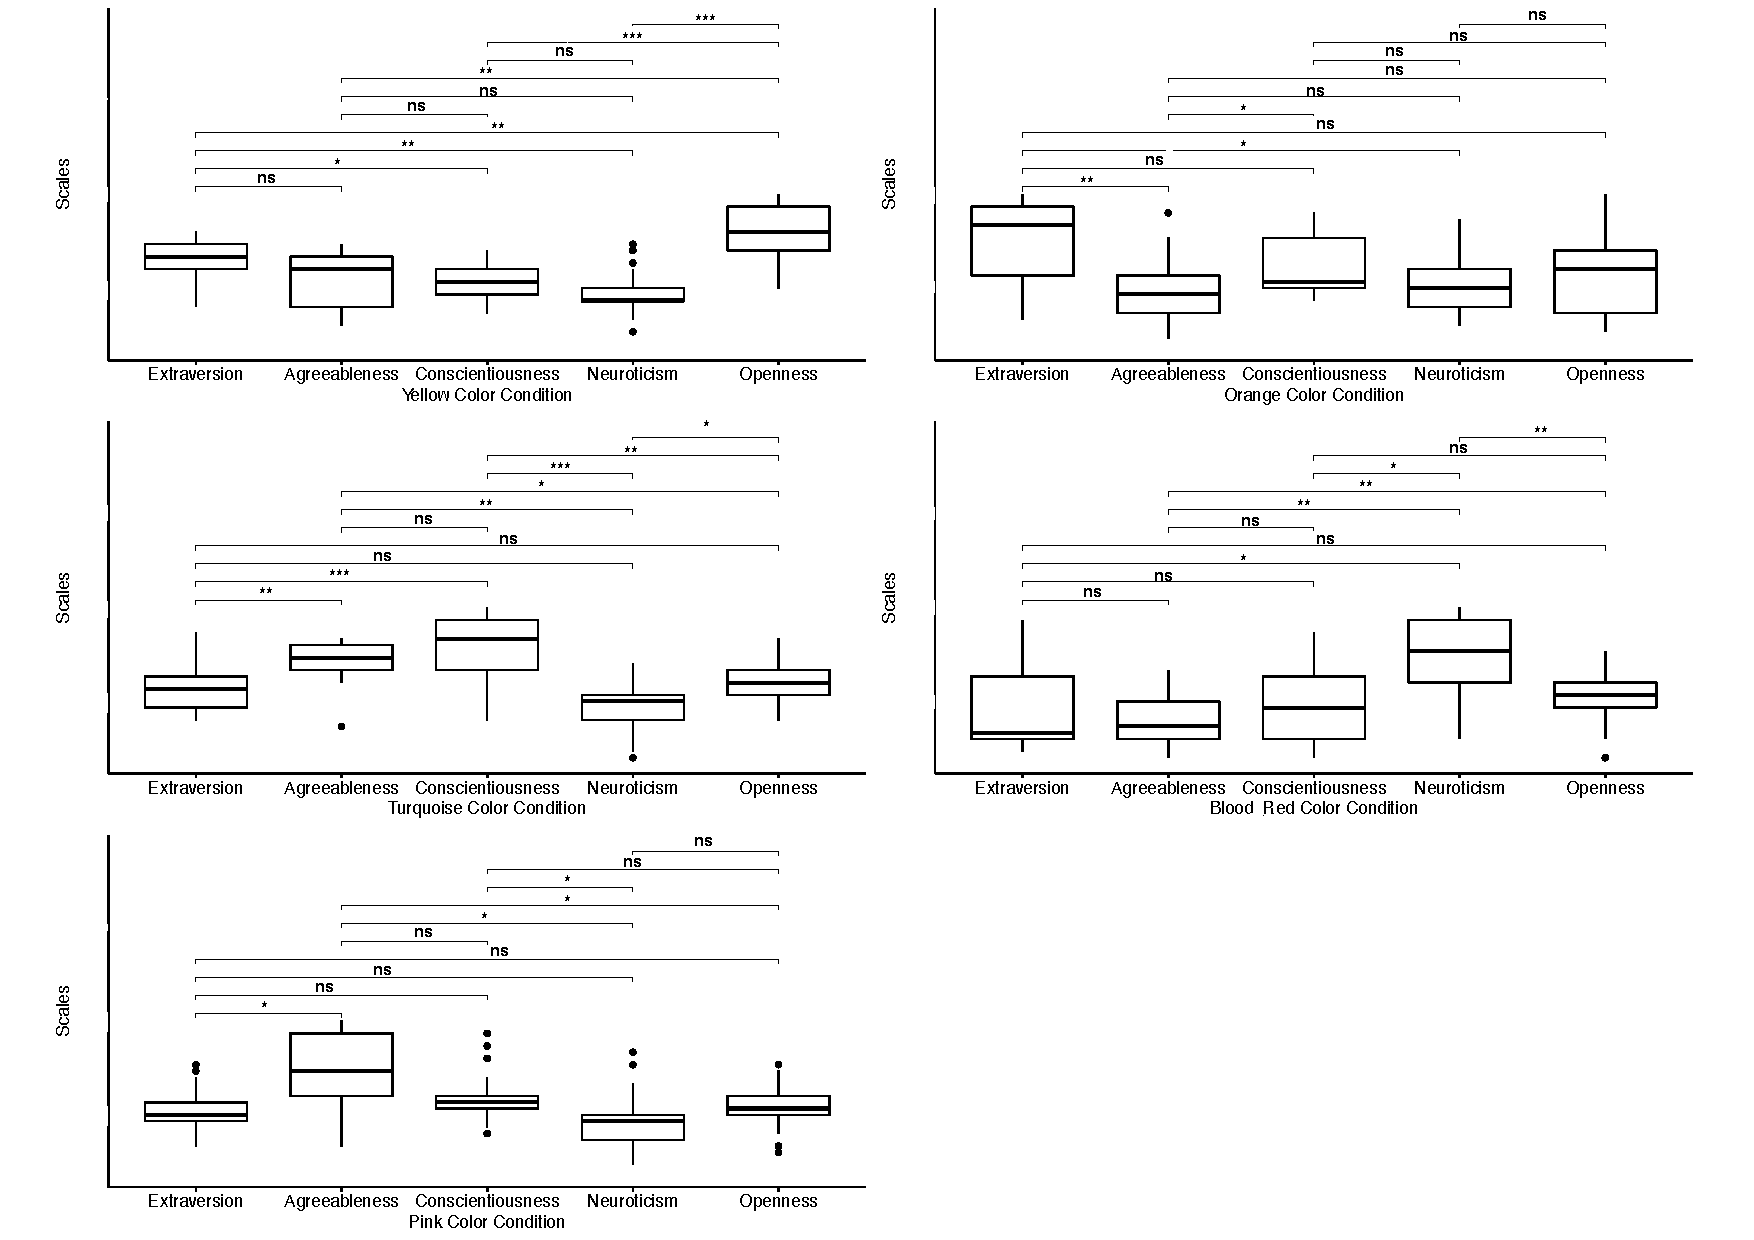
\includegraphics[scale=0.45]{Study2(M-T).pdf}
    \caption{A boxplot for Mascot-Lamp interaction in Study-1}
    \label{fig:MT2}
\end{figure}

% TODO: Table median (values)
% TODO: Figure p-values
% TODO: p-value, df=?
